\documentclass[a4paper]{article}

\usepackage[utf8]{inputenc}
\usepackage[english]{babel}
\usepackage{amsmath,amsfonts,amssymb,amsthm,amscd}
\usepackage{mathtools}
\usepackage{color}
\usepackage{parskip}
\usepackage{fancyhdr}
\usepackage{nicefrac}
\usepackage{cite}
\usepackage{graphicx}
\usepackage{subcaption}
\usepackage[table]{xcolor}
\usepackage{tikz}
\usetikzlibrary{decorations.markings}
\usetikzlibrary{calc}
\usetikzlibrary{shapes.misc}
\usetikzlibrary{hobby} 
\tikzstyle{hackennode}=[draw,circle,fill=white,inner sep=0,minimum size=4pt]
\tikzstyle{hackenline}=[line width=3pt]
\usepackage{scalefnt}
\usepackage[all]{xy}
\usepackage{pgfplots}
\usepackage{listings}
\usepackage{setspace}
\usepackage{siunitx}
\usepackage{float}
\usepackage{textcomp}
\usepackage{caption}
\usepackage[nottoc,notlot,notlof]{tocbibind}
\usepackage{mdframed}

\newcommand{\C}{\mathbb C}
\newcommand{\R}{\mathbb R}
\newcommand{\deriv}[2]{\frac{\mathrm{d}#1}{\mathrm{d}#2}}
\newcommand{\dderiv}[2]{\frac{\mathrm{d^2}#1}{\mathrm{d}#2^2}}
\newcommand{\dint}{\,\mathrm{d}}
\newcommand{\ve}[1]{\mathbf{#1}}

\theoremstyle{plain}
\newtheorem{thm1}{Theorem}
\newtheorem{lem1}[thm1]{Lemma}
\newtheorem{cor}[thm1]{Corollary}
\newtheorem{prop}[thm1]{Proposition}
\newtheorem{ctex}[thm1]{Counterexample}

\theoremstyle{definition}
\newtheorem{ex1}[thm1]{Example}
\newtheorem{remrk}[thm1]{Remark}
\newtheorem{defn1}[thm1]{Definition}


\usepackage[many]{tcolorbox}

\newtcolorbox{ex}[2][]{%
  enhanced,frame hidden,interior hidden,
  arc=10pt,outer arc=10pt,borderline={3pt}{2pt}{dashed,thick},borderline={3pt}{-2pt}{dashed,thick},
  before upper={#2\begin{ex1}},after upper={\end{ex1}}
}
\newtcolorbox{proof2}[2][]{%
  enhanced,breakable,frame hidden,interior hidden,
  arc=0pt,outer arc=0pt,borderline={0.5pt}{-0pt}{dashed},
  before upper={\begin{proof}[\textbf{#2}]},after upper={\end{proof}}
}

\newenvironment{defn}
  {\begin{mdframed}\begin{defn1}}
  {\end{defn1}\end{mdframed}}
\newenvironment{thm}
  {\begin{mdframed}\begin{thm1}}
  {\end{thm1}\end{mdframed}}
\newenvironment{lem}
  {\begin{mdframed}[nobreak=true]\begin{lem1}}
  {\end{lem1}\end{mdframed}}

\usepackage[a4paper, total={5.6in, 8.2in}]{geometry}
\usepackage{wrapfig}
\usepackage[labelfont=bf]{caption}
\usepackage{rotating}

\allowdisplaybreaks
\usepackage{lipsum}
\usepackage{hhline}

\usepackage{rotating}

\begin{document}
\pagenumbering{gobble}% Remove page numbers (and reset to 1)
\title{Exploiting Temporal Difference for Energy Disaggregation via Discriminative Sparse Coding}
%\date{2013-12-11}
\author{Eric Leijonmarck\\
\texttt{ericle@kth.se}}
\begin{titlepage}
\begin{center}

\makeatletter

% Upper part of the page. The '~' is needed because \\
% only works if a paragraph has started.

%\begin{figure}[h!]
%  \centering
%    \includegraphics[width=0.3\textwidth]{KTH}
%\end{figure}
%~\\~\\
\textsc{{\LARGE KTH Royal Institute of Technology}
\\[0.3cm]
{\large Department of Mathematics}
\\[0.7cm]
{\Large SF299X, Master's Thesis}}\\[0.5cm]

% Title
\noindent
\rule{\linewidth}{0.2mm}
{ \begin{spacing}{1.5} \Huge \bfseries \@title \end{spacing} }
\noindent
\rule{\linewidth}{0.2mm}\\[1.5cm]

% Author and supervisor
\begin{minipage}{0.4\textwidth}
\begin{flushleft} \large
\emph{Author:}\\
\@author
\end{flushleft}
\end{minipage}
\begin{minipage}{0.4\textwidth}
\begin{flushright} \large
\emph{Examiner} \\
Timo Koski\\
\texttt{tjtkoski@kth.se}
\end{flushright}
\end{minipage}

\vfill

% Bottom of the page
{\large \@date}

\makeatother

\end{center}
\end{titlepage}


\begin{abstract}
\noindent
This thesis analyzes one hour based energy disaggregation using Sparse Coding by exploiting temporal differences. Energy disaggregation is the task of taking a whole-home energy signal and separating it into its component appliances. Studies have shown that having device-level energy information can cause users to conserve significant amounts of energy, but current electricity meters only report whole-home data. Thus, developing algorithmic methods for disaggregation presents a key technical challenge in the effort to maximize energy conservation. In Energy Disaggregation or sometimes called Non-Intrusive Load Monitoring (NILM) most approaches are based on high frequent monitored appliances, while households only measure their consumption via smart-meters, which only account for one-hour measurements. This thesis aims at implementing key algorithms from J. Zico Kotler, Siddarth Batra and Andrew Ng paper "Energy Disaggregation via Discriminative Sparse Coding" and try to replicate the results by exploiting temporal differences that occur when dealing with time series data. The implementation was successful, but the results were inconclusive when dealing with large datasets, as the algorithm was too computationally heavy for the resources available. The work was performed at the Swedish company Greenely, who develops visualizations based on gamification for energy bills via a mobile application.


%\\
%It is shown that blah blah
%It is shown that all such games are numbers and that the dominating game options are to remove elements not lower than any other element of the same color. 
%\\
%In particular, the thesis show that ...
%In particular, the thesis concerns games played on posets that are chess-colored Young diagrams. It is shown that it is easy to compute the value for any such game with $\le3$ rows by proving a proposed formula for computing the value.
\end{abstract}
%~\\\\
\newpage
\rule{\linewidth}{0.2mm}
{\begin{spacing}{1.5} \centering{\LARGE\bfseries  Utforskande av tempor\"ara skillnader f\"or Energi Disaggregering med Sparse Coding} \end{spacing}}
\rule{\linewidth}{0.2mm}\\[1.5cm]

\renewcommand{\abstractname}{Sammanfattning}
\begin{abstract}
\noindent
I den h\"ar uppsatsen analyseras Energi Disaggregering med hjälp av Sparse Coding genom att utforska temporala skillnader på en timbaserade data. Studer har visat att presentera information p\r{a} apparat nivå kan det g\"ora att anv\"andare utnyttjar mindre energi i hemmen d\"ar man idag bara presenterar hela hush\r{a}llets anv\"andning. Denna uppsats har som mål att implementera och utveckla de algoritmer J. Zico Kotler, Siddarth Batra and Andrew Ng presenterar i deras artikel "Energy Disaggregation via Discriminative Sparse Coding", genom att anv\"anda sig utav de tempor\"ara skillnader som uppstår inom tidsseriedata. I uppsatsen uppnåde man ett s\"amre resultat, d\"ar datakraften var inte tillr\"acklig f\"or att utnyttja datan på b\"asta s\"att. Arbetet var utf\"ort på Greenely, ett f\"oretag som utvecklar visualiseringar utav elr\"akningen via en mobilapplikation.
%I synnerhet fokuserar denna uppsats p\r{a} spel som spelas p\r{a} pom\"angder som \"ar schackf\"argade Young-diagram. Det visas att det \"ar l\"att att ber\"akna v\"ardet p\r{a} alla s\r{a}dana spel med $\le3$ rader genom att bevisa en f\"oreslagen formel f\"or att r\"akna ut v\"ardet.
\end{abstract}
\newpage
%\newpage
\renewcommand{\abstractname}{Acknowledgements}
\begin{abstract}
\noindent
I would like to express my gratitude to my supervisor at KTH Royal Institute of Technology, Timo Koski, for his valuable scientific support and continuous interest and dedication throughout the process of this thesis. I would also like to thank Pawel Herman, for his interest in my thesis. I take this opportunity to express my sincerest gratitude to all of the team members at Greenely for providing me with the facilities, equipment, support and their knowledge within the field.
\end{abstract}
%• Abstract: the complete report condensed to less than half a page. Do not forget the
%results and do not refer to the content in the report.
\newpage

\tableofcontents
%Process
% Independently plan and carry out the project within agreed time frames, show good initiative and be open to supervision and critique. Independently identify one’s own need for new knowledge and acquire this knowledge. Show a good ability to adopt the perspective of another’s work and formulate relevant and constructive critique.
%Engineering
% From problems/inquiries and methodology, show a very good ability to apply engineering-related and scientific skills like problem formulation, modelling, analysis, development and evaluation in a systematic way. Where this is relevant, show awareness of societal and ethical aspects, including economically, socially, and ecologically sustainable development.

% overview commands
\newcommand{\intOverview}{This section describes the motivation behind this thesis, it also gives a brief introduction to energy disaggregation and its challenges and future prospects.}
\newcommand{\preOverview}{This section presents a brief overview of the mathematical background behind Optimization, Machine Learning and Artificial Neural Networks (ANN) to eventually go into Sparse Coding with two examples in computer vision and speech recognition.}
\newcommand{\proOverview}{In this section we describe what is demanded from the solution and what the thesis aim at achieve as well as some useful simplifications made for the thesis.}
\newcommand{\fabOverview}{In this section we talk about the dataset used and the data pre-processing done for usability. Here we also make a complete outline of the Discriminative Disaggregation via Sparse Coding (DDSC) algorithm, as well as the implementation.}
\newcommand{\resOverview}{This section presents the performed experiments, along with their respective results. We first present results based on subset to prove that the algorithm works properly on a small subset. Next we present results on different temporal subsets of the data. We then present predicted energy profiles and total energy profiles, then showing the learned basis functions and furthermore error and accuracy results. Finally, showing the evolution of the accuracy and error for the different settings.}
\newcommand{\conOverview}{This section discusses and concludes the methods and results given by this paper, as well as future research and improvements that could be made to the implementation.}

\newpage
\pagenumbering{arabic}% Arabic page numbers (and reset to 1)
\section{Introduction}
%What is the purpose? What is the context? What has been done before?
%How does this differ from earlier work? Explain the structure of the report.
In this section we will give an informal introduction of a partizan two-player game played on black-and-white-colored posets. The game is played by removing poset elements of your color, with the result that all greater elements in the poset are removed as well. The game ends when  one of the players has no elements left to remove. This player then loses.
\\
An example of such a game is provided below in Example \ref{ex:game}.
\\
\begin{ex}{}
\label{ex:game}
An example of a partizan element removal game played on a colored poset and an example of gameplay on this game.
\begin{figure}[H]
\centering
$
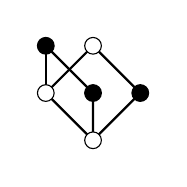
\begin{tikzpicture}[baseline=-0.65ex,scale=.2]
  \draw[thick] (0,-3) -- (-3,0) -- (0,3) -- (3,0) -- (0,-3);
  \draw[thick] (0,-3) -- (0,0) -- (-3,3);
  \draw[thick] (-3,0) -- (-3,3);
  \node (zero) at (0,-3) {\tikz\draw[black,fill=white] (0,0) circle (.7ex);};
  \node (1) at (-3,0) {\tikz\draw[black,fill=white] (0,0) circle (.7ex);};
  \node (2) at (0,0) {\tikz\draw[black,fill=black] (0,0) circle (.7ex);};
  \node (3) at (3,0) {\tikz\draw[black,fill=black] (0,0) circle (.7ex);};
  \node (4) at (-3,3) {\tikz\draw[black,fill=black] (0,0) circle (.7ex);};
  \node (5) at (0,3) {\tikz\draw[black,fill=white] (0,0) circle (.7ex);};
\end{tikzpicture}
=\left\{
\underbrace{
\emptyset
,

\begin{tikzpicture}[baseline=-0.65ex,scale=.2]
  \draw[thick] (0,-1) -- (3,2);
  \draw[thick] (0,-1) -- (0,2);
  \node (zero) at (0,-1) {\tikz\draw[black,fill=white] (0,0) circle (.7ex);};
  \node (2) at (0,2) {\tikz\draw[black,fill=black] (0,0) circle (.7ex);};
  \node (3) at (3,2) {\tikz\draw[black,fill=black] (0,0) circle (.7ex);};
\end{tikzpicture}
,
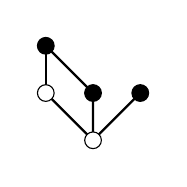
\begin{tikzpicture}[baseline=-0.65ex,scale=.2]
  \draw[thick] (0,-3) -- (-3,0);
  \draw[thick] (0,-3) -- (3,0);
  \draw[thick] (0,-3) -- (0,0) -- (-3,3);
  \draw[thick] (-3,0) -- (-3,3);
  \node (zero) at (0,-3) {\tikz\draw[black,fill=white] (0,0) circle (.7ex);};
  \node (1) at (-3,0) {\tikz\draw[black,fill=white] (0,0) circle (.7ex);};
  \node (2) at (0,0) {\tikz\draw[black,fill=black] (0,0) circle (.7ex);};
  \node (3) at (3,0) {\tikz\draw[black,fill=black] (0,0) circle (.7ex);};
  \node (4) at (-3,3) {\tikz\draw[black,fill=black] (0,0) circle (.7ex);};
\end{tikzpicture}
}_{\text{Left player options}}
\middle|
\underbrace{
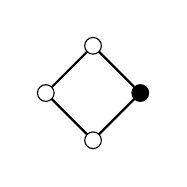
\begin{tikzpicture}[baseline=-0.65ex,scale=.2]
  \draw[thick] (0,-3) -- (-3,0) -- (0,3) -- (3,0) -- (0,-3);
  \node (zero) at (0,-3) {\tikz\draw[black,fill=white] (0,0) circle (.7ex);};
  \node (1) at (-3,0) {\tikz\draw[black,fill=white] (0,0) circle (.7ex);};
  \node (3) at (3,0) {\tikz\draw[black,fill=black] (0,0) circle (.7ex);};
  \node (5) at (0,3) {\tikz\draw[black,fill=white] (0,0) circle (.7ex);};
\end{tikzpicture}
,
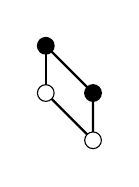
\begin{tikzpicture}[baseline=-0.65ex,scale=.2]
  \draw[thick] (0,-3) -- (-3,0);
  \draw[thick] (0,-3) -- (0,0) -- (-3,3);
  \draw[thick] (-3,0) -- (-3,3);
  \node (zero) at (0,-3) {\tikz\draw[black,fill=white] (0,0) circle (.7ex);};
  \node (1) at (-3,0) {\tikz\draw[black,fill=white] (0,0) circle (.7ex);};
  \node (2) at (0,0) {\tikz\draw[black,fill=black] (0,0) circle (.7ex);};
  \node (4) at (-3,3) {\tikz\draw[black,fill=black] (0,0) circle (.7ex);};
\end{tikzpicture}
,
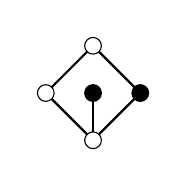
\begin{tikzpicture}[baseline=-0.65ex,scale=.2]
  \draw[thick] (0,-3) -- (-3,0) -- (0,3) -- (3,0) -- (0,-3);
  \draw[thick] (0,-3) -- (0,0);
  \node (zero) at (0,-3) {\tikz\draw[black,fill=white] (0,0) circle (.7ex);};
  \node (1) at (-3,0) {\tikz\draw[black,fill=white] (0,0) circle (.7ex);};
  \node (2) at (0,0) {\tikz\draw[black,fill=black] (0,0) circle (.7ex);};
  \node (3) at (3,0) {\tikz\draw[black,fill=black] (0,0) circle (.7ex);};
  \node (5) at (0,3) {\tikz\draw[black,fill=white] (0,0) circle (.7ex);};
\end{tikzpicture}
}_{\text{Right player options}}
\right\}
$
\caption{Example of a colored poset element removal game.}
\label{fig:posetgameex}
\end{figure}
\begin{figure}[H]
\centering
$
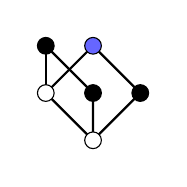
\begin{tikzpicture}[baseline=-0.65ex,scale=.2]
  \draw[thick] (0,-3) -- (-3,0) -- (0,3) -- (3,0) -- (0,-3);
  \draw[thick] (0,-3) -- (0,0) -- (-3,3);
  \draw[thick] (-3,0) -- (-3,3);
  \node (zero) at (0,-3) {\tikz\draw[black,fill=white] (0,0) circle (.7ex);};
  \node (1) at (-3,0) {\tikz\draw[black,fill=white] (0,0) circle (.7ex);};
  \node (2) at (0,0) {\tikz\draw[black,fill=black] (0,0) circle (.7ex);};
  \node (3) at (3,0) {\tikz\draw[black,fill=black] (0,0) circle (.7ex);};
  \node (4) at (-3,3) {\tikz\draw[black,fill=black] (0,0) circle (.7ex);};
  \node (5) at (0,3) {\tikz\draw[black,fill=blue!60] (0,0) circle (.7ex);};
\end{tikzpicture}
\overset{L}{\longrightarrow}
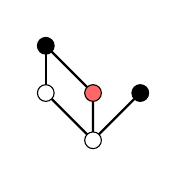
\begin{tikzpicture}[baseline=-0.65ex,scale=.2]
  \draw[thick] (0,-3) -- (-3,0);
  \draw[thick] (0,-3) -- (3,0);
  \draw[thick] (0,-3) -- (0,0) -- (-3,3);
  \draw[thick] (-3,0) -- (-3,3);
  \node (zero) at (0,-3) {\tikz\draw[black,fill=white] (0,0) circle (.7ex);};
  \node (1) at (-3,0) {\tikz\draw[black,fill=white] (0,0) circle (.7ex);};
  \node (2) at (0,0) {\tikz\draw[black,fill=red!60] (0,0) circle (.7ex);};
  \node (3) at (3,0) {\tikz\draw[black,fill=black] (0,0) circle (.7ex);};
  \node (4) at (-3,3) {\tikz\draw[black,fill=black] (0,0) circle (.7ex);};
\end{tikzpicture}
\overset{R}{\longrightarrow}
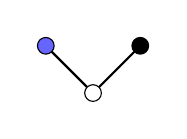
\begin{tikzpicture}[baseline=-0.65ex,scale=.2]
  \draw[thick] (0,-3) -- (-3,0);
  \draw[thick] (0,-3) -- (3,0);
  \node (zero) at (0,-3) {\tikz\draw[black,fill=white] (0,0) circle (.7ex);};
  \node (1) at (-3,0) {\tikz\draw[black,fill=blue!60] (0,0) circle (.7ex);};
  \node (3) at (3,0) {\tikz\draw[black,fill=black] (0,0) circle (.7ex);};
\end{tikzpicture}
\overset{L}{\longrightarrow}

\begin{tikzpicture}[baseline=-0.65ex,scale=.2]
  \draw[thick] (0,-3) -- (3,0);
  \node (zero) at (0,-3) {\tikz\draw[black,fill=white] (0,0) circle (.7ex);};
  \node (3) at (3,0) {\tikz\draw[black,fill=red!60] (0,0) circle (.7ex);};
\end{tikzpicture}
\overset{R}{\longrightarrow}
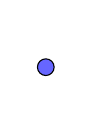
\begin{tikzpicture}[baseline=-0.65ex,scale=.2]
  \node (zero) at (0,-3) {\tikz\draw[black,fill=blue!60] (0,0) circle (.7ex);};
\end{tikzpicture}
\overset{L}{\longrightarrow}
%\emptyset
$
\caption{Example of gameplay on the game in Figure \ref{fig:posetgameex} where Left player wins. Play moves are highlighted with blue (Left) and red (Right).}
\end{figure}
\end{ex}
~\\
In particular, this thesis will focus on games played on \emph{chess-colored} posets, where the posets are in the form of \emph{Young diagrams}. An example of a chess-colored Young diagram and a game played on this Young diagram is provided in Example \ref{ex:younggameplay}.
\begin{ex}{}
\label{ex:younggameplay}
An example of a chess-colored Young diagram and an example of a gameplay on this Young diagram.
\begin{figure}[H]
\centering
\begin{tabular}{ | c | c | c | c | c | c | c |}
\hline
~&\cellcolor[gray]{0}&~&\cellcolor[gray]{0}&~&\cellcolor[gray]{0}&~\\
\hline
\cellcolor[gray]{0}&~&\cellcolor[gray]{0}&~&\cellcolor[gray]{0}\\
\cline{1-5}
~&\cellcolor[gray]{0}\\
\cline{1-2}
\cellcolor[gray]{0}&~\\
\cline{1-2}
~\\
\cline{1-1}
\end{tabular}
\captionof{figure}{Example of a chess-colored Young diagram.}
\label{fig:chessyoungex}
\end{figure}
\begin{figure}[H]
\centering
$
\begin{tabular}{ | c | c | c | c | c | c | c |}
\hline
~&\cellcolor[gray]{0}&~&\cellcolor[gray]{0}&\cellcolor{blue!60}&\cellcolor[gray]{0}&~\\
\hline
\cellcolor[gray]{0}&~&\cellcolor[gray]{0}&~&\cellcolor[gray]{0}\\
\cline{1-5}
~&\cellcolor[gray]{0}\\
\cline{1-2}
\cellcolor[gray]{0}&~\\
\cline{1-2}
~\\
\cline{1-1}
\end{tabular}
\overset{L}{\longrightarrow}
\begin{tabular}{ | c | c | c | c |}
\hline
~&\cellcolor[gray]{0}&~&\cellcolor[gray]{0}\\
\hline
\cellcolor{red!60}&~&\cellcolor[gray]{0}&~\\
\cline{1-4}
~&\cellcolor[gray]{0}\\
\cline{1-2}
\cellcolor[gray]{0}&~\\
\cline{1-2}
~\\
\cline{1-1}
\end{tabular}
\overset{R}{\longrightarrow}
\begin{tabular}{ | c | c | c | c |}
\hline
\cellcolor{blue!60}&\cellcolor[gray]{0}&~&\cellcolor[gray]{0}\\
\hline
\end{tabular}
\overset{L}{\longrightarrow}
\emptyset
$
\captionof{figure}{Example of gameplay on the chess-colored Young diagram of Figure \ref{fig:chessyoungex} where Left player wins. Play moves are highlighted with blue (Left) and red (Right).}
\label{fig:chessyounggameplay}
\end{figure}
\end{ex}
~\\
For these games in general, we will show that they are all surreal numbers, and that, given some properties, they always are valued between 0 and 1. %We will also show that games played on \emph{forest posets} are equivalent to games of \emph{Blue-Red Hackenbush}.
\\
Finally, for games played on chess-colored Young diagrams with $\le3$ rows, we will show that the value is easy to compute by proving that they can be computed with a given formula.
\\\\
First a brief background of poset games will be covered.
\subsection{Background}
A poset game is an element-removal game played on a poset, where a player selects an element and removes this element and all greater elements. A poset game can be both impartial (if it is not colored) and partizan (if it is colored, i.e., each element has a color which specifies who can select and remove it). It is known that the problem of deciding the winner of an impartial uncolored poset game is \textsf{PSPACE}-complete\cite{grier2013}.
\\\\
The simplest possible impartial poset game is the one played on a collection of one-dimensional chain posets, also known as \emph{Nim}. The game of Nim is played by removing a number of elements from one of multiple piles of elements. The player removing the last element wins the game. For a more intuitive understanding of Nim, an example of a gameplay on a game of Nim is provided in Example \ref{ex:nim}.
\begin{ex}{}
\label{ex:nim}
An example gameplay on a game of Nim.
\begin{figure}[H]
\centering
$
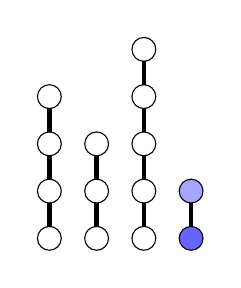
\begin{tikzpicture}[baseline=-0.65ex,scale=.2]
  \draw[ultra thick] (-2,-3) -- (-2,6);
  \draw[ultra thick] (1,-3) -- (1,3);
  \draw[ultra thick] (4,-3) -- (4,9);
  \draw[ultra thick] (7,-3) -- (7,0);
  \node (11) at (-2,-3) {\tikz\draw[black,fill=white] (0,0) circle (1ex);};
  \node (12) at (-2,0) {\tikz\draw[black,fill=white] (0,0) circle (1ex);};
  \node (13) at (-2,3) {\tikz\draw[black,fill=white] (0,0) circle (1ex);};
  \node (14) at (-2,6) {\tikz\draw[black,fill=white] (0,0) circle (1ex);};
  \node (21) at (1,-3) {\tikz\draw[black,fill=white] (0,0) circle (1ex);};
  \node (22) at (1,0) {\tikz\draw[black,fill=white] (0,0) circle (1ex);};
  \node (23) at (1,3) {\tikz\draw[black,fill=white] (0,0) circle (1ex);};
  \node (31) at (4,-3) {\tikz\draw[black,fill=white] (0,0) circle (1ex);};
  \node (32) at (4,0) {\tikz\draw[black,fill=white] (0,0) circle (1ex);};
  \node (33) at (4,3) {\tikz\draw[black,fill=white] (0,0) circle (1ex);};
  \node (34) at (4,6) {\tikz\draw[black,fill=white] (0,0) circle (1ex);};
  \node (35) at (4,9) {\tikz\draw[black,fill=white] (0,0) circle (1ex);};
  \node (41) at (7,-3) {\tikz\draw[black,fill=blue!60] (0,0) circle (1ex);};
  \node (42) at (7,0) {\tikz\draw[black,fill=blue!35] (0,0) circle (1ex);};
\end{tikzpicture}
\overset{L}{\longrightarrow}
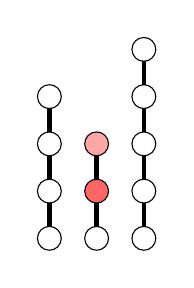
\begin{tikzpicture}[baseline=-0.65ex,scale=.2]
  \draw[ultra thick] (-2,-3) -- (-2,6);
  \draw[ultra thick] (1,-3) -- (1,3);
  \draw[ultra thick] (4,-3) -- (4,9);
  \node (11) at (-2,-3) {\tikz\draw[black,fill=white] (0,0) circle (1ex);};
  \node (12) at (-2,0) {\tikz\draw[black,fill=white] (0,0) circle (1ex);};
  \node (13) at (-2,3) {\tikz\draw[black,fill=white] (0,0) circle (1ex);};
  \node (14) at (-2,6) {\tikz\draw[black,fill=white] (0,0) circle (1ex);};
  \node (21) at (1,-3) {\tikz\draw[black,fill=white] (0,0) circle (1ex);};
  \node (22) at (1,0) {\tikz\draw[black,fill=red!60] (0,0) circle (1ex);};
  \node (23) at (1,3) {\tikz\draw[black,fill=red!35] (0,0) circle (1ex);};
  \node (31) at (4,-3) {\tikz\draw[black,fill=white] (0,0) circle (1ex);};
  \node (32) at (4,0) {\tikz\draw[black,fill=white] (0,0) circle (1ex);};
  \node (33) at (4,3) {\tikz\draw[black,fill=white] (0,0) circle (1ex);};
  \node (34) at (4,6) {\tikz\draw[black,fill=white] (0,0) circle (1ex);};
  \node (35) at (4,9) {\tikz\draw[black,fill=white] (0,0) circle (1ex);};
\end{tikzpicture}
\overset{R}{\longrightarrow}
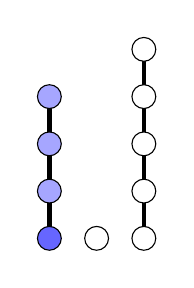
\begin{tikzpicture}[baseline=-0.65ex,scale=.2]
  \draw[ultra thick] (-2,-3) -- (-2,6);
  \draw[ultra thick] (4,-3) -- (4,9);
  \node (11) at (-2,-3) {\tikz\draw[black,fill=blue!60] (0,0) circle (1ex);};
  \node (12) at (-2,0) {\tikz\draw[black,fill=blue!35] (0,0) circle (1ex);};
  \node (13) at (-2,3) {\tikz\draw[black,fill=blue!35] (0,0) circle (1ex);};
  \node (14) at (-2,6) {\tikz\draw[black,fill=blue!35] (0,0) circle (1ex);};
  \node (21) at (1,-3) {\tikz\draw[black,fill=white] (0,0) circle (1ex);};
  \node (31) at (4,-3) {\tikz\draw[black,fill=white] (0,0) circle (1ex);};
  \node (32) at (4,0) {\tikz\draw[black,fill=white] (0,0) circle (1ex);};
  \node (33) at (4,3) {\tikz\draw[black,fill=white] (0,0) circle (1ex);};
  \node (34) at (4,6) {\tikz\draw[black,fill=white] (0,0) circle (1ex);};
  \node (35) at (4,9) {\tikz\draw[black,fill=white] (0,0) circle (1ex);};
\end{tikzpicture}
\overset{L}{\longrightarrow}
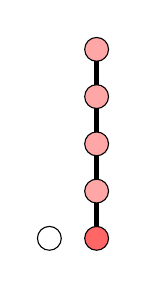
\begin{tikzpicture}[baseline=-0.65ex,scale=.2]
  \draw[ultra thick] (4,-3) -- (4,9);
  \node (21) at (1,-3) {\tikz\draw[black,fill=white] (0,0) circle (1ex);};
  \node (31) at (4,-3) {\tikz\draw[black,fill=red!60] (0,0) circle (1ex);};
  \node (32) at (4,0) {\tikz\draw[black,fill=red!35] (0,0) circle (1ex);};
  \node (33) at (4,3) {\tikz\draw[black,fill=red!35] (0,0) circle (1ex);};
  \node (34) at (4,6) {\tikz\draw[black,fill=red!35] (0,0) circle (1ex);};
  \node (35) at (4,9) {\tikz\draw[black,fill=red!35] (0,0) circle (1ex);};
\end{tikzpicture}
\overset{R}{\longrightarrow}

\begin{tikzpicture}[baseline=-0.65ex,scale=.2]
  \node (21) at (0,-3) {\tikz\draw[black,fill=blue!60] (0,0) circle (1ex);};
\end{tikzpicture}
\overset{L}{\longrightarrow}
\begin{tikzpicture}[baseline=-0.0ex]
  \node at (0,-0.55) {$\emptyset$};
\end{tikzpicture}
%\emptyset
$
\caption{Example of gameplay on a game of Nim where Left player wins. Play moves are highlighted with blue (Left) and red (Right).}
\end{figure}
\end{ex}
~\\
Another impartial poset game is the game \emph{Chomp}, more thoroughly introduced in Section \ref{section:chomp}. A game of Chomp can be represented by a poset game with a two-dimensional $n\times m$ lattice poset, $n,m>0$ integers, with the bottom element removed, as illustrated in Figure \ref{fig:chompposet}.

\begin{figure}[H]
\centering
\begin{subfigure}{0.25\textwidth}
\begin{tabular}{ | c | c | c | c | c |}
\hline
~&~&~&~&~\\
\hline
~&~&~&~&~\\
\hline
~&~&~&~&~\\
\hline
~&~&~&~&~\\
\hline
~&~&~&~&~\\
\hline
~&~&~&~&~\\
\hline
\cellcolor{red}&~&~&~&~\\
\hline
\end{tabular}
\hfill$\Longleftrightarrow$
\end{subfigure}
\begin{subfigure}{0.4\textwidth}
\centering
%\begin{turn}{45}
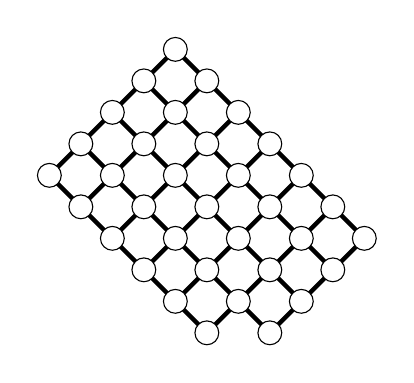
\begin{tikzpicture}[scale=.4]
  \draw[ultra thick] (1,0) -- (4,3);
  \draw[ultra thick] (-1,0) -- (3,4);
  \draw[ultra thick] (-2,1) -- (2,5);
  \draw[ultra thick] (-3,2) -- (1,6);
  \draw[ultra thick] (-4,3) -- (0,7);
  \draw[ultra thick] (-5,4) -- (-1,8);
  \draw[ultra thick] (-6,5) -- (-2,9);
  \draw[ultra thick] (-1,0) -- (-6,5);
  \draw[ultra thick] (1,0) -- (-5,6);
  \draw[ultra thick] (2,1) -- (-4,7);
  \draw[ultra thick] (3,2) -- (-3,8);
  \draw[ultra thick] (4,3) -- (-2,9);
  \node (12) at (1,0) {\tikz\draw[black,fill=white] (0,0) circle (1ex);};
  \node (13) at (2,1) {\tikz\draw[black,fill=white] (0,0) circle (1ex);};
  \node (14) at (3,2) {\tikz\draw[black,fill=white] (0,0) circle (1ex);};
  \node (21) at (4,3) {\tikz\draw[black,fill=white] (0,0) circle (1ex);};
  \node (12) at (-1,0) {\tikz\draw[black,fill=white] (0,0) circle (1ex);};
  \node (12) at (0,1) {\tikz\draw[black,fill=white] (0,0) circle (1ex);};
  \node (13) at (1,2) {\tikz\draw[black,fill=white] (0,0) circle (1ex);};
  \node (14) at (2,3) {\tikz\draw[black,fill=white] (0,0) circle (1ex);};
  \node (21) at (3,4) {\tikz\draw[black,fill=white] (0,0) circle (1ex);};
  \node (12) at (-2,1) {\tikz\draw[black,fill=white] (0,0) circle (1ex);};
  \node (12) at (-1,2) {\tikz\draw[black,fill=white] (0,0) circle (1ex);};
  \node (13) at (0,3) {\tikz\draw[black,fill=white] (0,0) circle (1ex);};
  \node (14) at (1,4) {\tikz\draw[black,fill=white] (0,0) circle (1ex);};
  \node (21) at (2,5) {\tikz\draw[black,fill=white] (0,0) circle (1ex);};
  \node (12) at (-3,2) {\tikz\draw[black,fill=white] (0,0) circle (1ex);};
  \node (12) at (-2,3) {\tikz\draw[black,fill=white] (0,0) circle (1ex);};
  \node (13) at (-1,4) {\tikz\draw[black,fill=white] (0,0) circle (1ex);};
  \node (14) at (0,5) {\tikz\draw[black,fill=white] (0,0) circle (1ex);};
  \node (21) at (1,6) {\tikz\draw[black,fill=white] (0,0) circle (1ex);};
  \node (12) at (-4,3) {\tikz\draw[black,fill=white] (0,0) circle (1ex);};
  \node (12) at (-3,4) {\tikz\draw[black,fill=white] (0,0) circle (1ex);};
  \node (13) at (-2,5) {\tikz\draw[black,fill=white] (0,0) circle (1ex);};
  \node (14) at (-1,6) {\tikz\draw[black,fill=white] (0,0) circle (1ex);};
  \node (21) at (0,7) {\tikz\draw[black,fill=white] (0,0) circle (1ex);};
  \node (12) at (-5,4) {\tikz\draw[black,fill=white] (0,0) circle (1ex);};
  \node (12) at (-4,5) {\tikz\draw[black,fill=white] (0,0) circle (1ex);};
  \node (13) at (-3,6) {\tikz\draw[black,fill=white] (0,0) circle (1ex);};
  \node (14) at (-2,7) {\tikz\draw[black,fill=white] (0,0) circle (1ex);};
  \node (21) at (-1,8) {\tikz\draw[black,fill=white] (0,0) circle (1ex);};
  \node (12) at (-6,5) {\tikz\draw[black,fill=white] (0,0) circle (1ex);};
  \node (12) at (-5,6) {\tikz\draw[black,fill=white] (0,0) circle (1ex);};
  \node (13) at (-4,7) {\tikz\draw[black,fill=white] (0,0) circle (1ex);};
  \node (14) at (-3,8) {\tikz\draw[black,fill=white] (0,0) circle (1ex);};
  \node (21) at (-2,9) {\tikz\draw[black,fill=white] (0,0) circle (1ex);};
\end{tikzpicture}
%\end{turn}
\end{subfigure}
\captionof{figure}{A game of Chomp is equivalent to an impartial poset game.}
\label{fig:chompposet}
\end{figure}
While the game of Nim is solved\cite{bouton1901}, i.e., there is a known optimal strategy, there is not so much known about the game of Chomp in general. This also points out how the difficulty can differ for two classes of impartial poset games. Therefore, it is interesting to investigate the properties of \emph{partizan} poset games, i.e., games on colored posets.
\\
In general, there have been very few studies on partizan poset games. One class of partizan poset games that have been studied are \emph{pomax games}. A pomax game is played on a colored poset, where each player can remove only maximal elements of their own color. Examples of pomax games can be found in Figures \ref{fig:posetpomax} and \ref{fig:youngpomax}.
\begin{figure}[H]
\centering
$
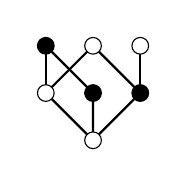
\begin{tikzpicture}[baseline=-0.65ex,scale=.2]
  \draw[thick] (0,-3) -- (-3,0) -- (0,3) -- (3,0) -- (0,-3);
  \draw[thick] (0,-3) -- (0,0) -- (-3,3);
  \draw[thick] (-3,0) -- (-3,3);
  \draw[thick] (3,0) -- (3,3);
  \node (zero) at (0,-3) {\tikz\draw[black,fill=white] (0,0) circle (.7ex);};
  \node (1) at (-3,0) {\tikz\draw[black,fill=white] (0,0) circle (.7ex);};
  \node (2) at (0,0) {\tikz\draw[black,fill=black] (0,0) circle (.7ex);};
  \node (3) at (3,0) {\tikz\draw[black,fill=black] (0,0) circle (.7ex);};
  \node (4) at (-3,3) {\tikz\draw[black,fill=black] (0,0) circle (.7ex);};
  \node (5) at (0,3) {\tikz\draw[black,fill=white] (0,0) circle (.7ex);};
  \node (6) at (3,3) {\tikz\draw[black,fill=white] (0,0) circle (.7ex);};
\end{tikzpicture}
=\left\{
\underbrace{
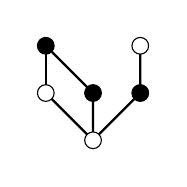
\begin{tikzpicture}[baseline=-0.65ex,scale=.2]
  \draw[thick] (0,-3) -- (-3,0);
  \draw[thick] (0,-3) -- (0,0) -- (-3,3);
  \draw[thick] (-3,0) -- (-3,3);
  \draw[thick] (0,-3) -- (3,0) -- (3,3);
  \node (zero) at (0,-3) {\tikz\draw[black,fill=white] (0,0) circle (.7ex);};
  \node (1) at (-3,0) {\tikz\draw[black,fill=white] (0,0) circle (.7ex);};
  \node (2) at (0,0) {\tikz\draw[black,fill=black] (0,0) circle (.7ex);};
  \node (3) at (3,0) {\tikz\draw[black,fill=black] (0,0) circle (.7ex);};
  \node (4) at (-3,3) {\tikz\draw[black,fill=black] (0,0) circle (.7ex);};
  \node (6) at (3,3) {\tikz\draw[black,fill=white] (0,0) circle (.7ex);};
\end{tikzpicture}
,
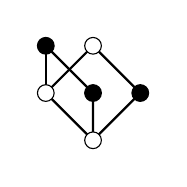
\begin{tikzpicture}[baseline=-0.65ex,scale=.2]
  \draw[thick] (0,-3) -- (-3,0) -- (0,3) -- (3,0) -- (0,-3);
  \draw[thick] (0,-3) -- (0,0) -- (-3,3);
  \draw[thick] (-3,0) -- (-3,3);
  \node (zero) at (0,-3) {\tikz\draw[black,fill=white] (0,0) circle (.7ex);};
  \node (1) at (-3,0) {\tikz\draw[black,fill=white] (0,0) circle (.7ex);};
  \node (2) at (0,0) {\tikz\draw[black,fill=black] (0,0) circle (.7ex);};
  \node (3) at (3,0) {\tikz\draw[black,fill=black] (0,0) circle (.7ex);};
  \node (4) at (-3,3) {\tikz\draw[black,fill=black] (0,0) circle (.7ex);};
  \node (5) at (0,3) {\tikz\draw[black,fill=white] (0,0) circle (.7ex);};
\end{tikzpicture}
}_{\text{Left player options}}
\;\middle|\;
\underbrace{
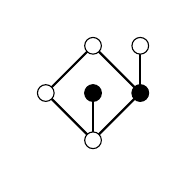
\begin{tikzpicture}[baseline=-0.65ex,scale=.2]
  \draw[thick] (0,-3) -- (-3,0) -- (0,3) -- (3,0) -- (0,-3);
  \draw[thick] (0,-3) -- (0,0);;
  \draw[thick] (3,0) -- (3,3);
  \node (zero) at (0,-3) {\tikz\draw[black,fill=white] (0,0) circle (.7ex);};
  \node (1) at (-3,0) {\tikz\draw[black,fill=white] (0,0) circle (.7ex);};
  \node (2) at (0,0) {\tikz\draw[black,fill=black] (0,0) circle (.7ex);};
  \node (3) at (3,0) {\tikz\draw[black,fill=black] (0,0) circle (.7ex);};
  \node (5) at (0,3) {\tikz\draw[black,fill=white] (0,0) circle (.7ex);};
  \node (6) at (3,3) {\tikz\draw[black,fill=white] (0,0) circle (.7ex);};
\end{tikzpicture}
}_{\text{Right player options}}
\right\}$
\caption{Example of an arbitrary pomax game.}
\label{fig:posetpomax}
\end{figure}
\begin{figure}[H]
\centering
$
\begin{tabular}{ | c | c | c | c | c |}
\hline
~&\cellcolor[gray]{0}&~&\cellcolor[gray]{0}&~\\
\hline
\cellcolor[gray]{0}&~&\cellcolor[gray]{0}\\
\cline{1-3}
~&\cellcolor[gray]{0}\\
\cline{1-2}
\cellcolor[gray]{0}&~\\
\cline{1-2}
\end{tabular}
=\left\{
\underbrace{
\begin{tabular}{ | c | c | c | c |}
\hline
~&\cellcolor[gray]{0}&~&\cellcolor[gray]{0}\\
\hline
\cellcolor[gray]{0}&~&\cellcolor[gray]{0}\\
\cline{1-3}
~&\cellcolor[gray]{0}\\
\cline{1-2}
\cellcolor[gray]{0}&~\\
\cline{1-2}
\end{tabular}
,
\begin{tabular}{ | c | c | c | c | c |}
\hline
~&\cellcolor[gray]{0}&~&\cellcolor[gray]{0}&~\\
\hline
\cellcolor[gray]{0}&~&\cellcolor[gray]{0}\\
\cline{1-3}
~&\cellcolor[gray]{0}\\
\cline{1-2}
\cellcolor[gray]{0}\\
\cline{1-1}
\end{tabular}
}_{\text{Left player options}}
\;\middle|\;
\underbrace{
\begin{tabular}{ | c | c | c | c | c |}
\hline
~&\cellcolor[gray]{0}&~&\cellcolor[gray]{0}&~\\
\hline
\cellcolor[gray]{0}&~\\
\cline{1-2}
~&\cellcolor[gray]{0}\\
\cline{1-2}
\cellcolor[gray]{0}&~\\
\cline{1-2}
\end{tabular}
}_{\text{Right player options}}
\right\}
$
\captionof{figure}{Example of a pomax game on a chess-colored Young diagram.}
\label{fig:youngpomax}
\end{figure}
It has been shown that all pomax games are integer valued\cite{j2013}, that it is easy to determine the value of pomax games played on trees or on chess-colored Young diagrams\cite{j2013} and that the problem of determining the winner of an arbitrary pomax game is \textsf{PSPACE}-complete\cite{js2014}.
\\\\
This thesis will focus on partizan poset games without the constraint of only being able to remove maximal elements, i.e., more similar to the gameplay of the regular poset games, only played on a colored poset. An illustrative example of this type of game is provided in Example \ref{ex:game}.

\newpage
%Preliminaries/Theory/Scientific Background/
\section{Preliminaries}
% Is there any useful theory? What are the methods used
% before for similar problems?

In this section a background of the theory behind the combinatorial games studied for this thesis is provided. In addition to this, the notation introduced here is used throughout the thesis. 

\subsection{Partially Ordered Sets}
This thesis is about a type of combinatorial games called \emph{poset games}. In order to be able to introduce the theory of these games, we must first define what a poset is.
\begin{defn}[Partially Ordered Sets{\cite[p.~278]{stanley2011}}]
A \emph{partially ordered set} (\emph{poset}) $(P,\le)$ is a set with a binary order relation $\le$ satisfying the following three axioms:
\begin{enumerate}
\item For all $t\in P$, $t\le t$ (reflexivity).
\item If $s\le t$ and $t\le s$,then $s=t$ (antisymmetry).
\item If $s\le t$ and $t\le u$,then $s\le u$ (transitivity).
\end{enumerate}
\end{defn}
~\\
We use the obvious notation $t\ge s$ to mean $s\le t$, $s<t$ to mean $s\le t$ and $s\ne t$, and $t>s$ to mean $s<t$. We say that two elements $s$ and $t$ of $P$ are \emph{comparable} if $s\le t$ or $t\le s$, otherwise $s$ and $t$ are \emph{incomparable}.
\\
We define an \emph{interval} $[p,q]$ of a poset to be $\{x\in P\;|\;p\le x\le q\}$. We say that $v$ covers $u$ if $[u,v]=\{u,v\}$, and we denote this by $u\lessdot v$.
\\\\
In a partizan element removal game, every element must have a color.
%\\
\begin{defn}[Colored Posets]
A \emph{colored poset} is a poset where each element has a color of either black or white.
\end{defn}
\begin{ex}{}
\label{ex:posets}
An example of a regular and a colored poset. %The elements higher up are greater than those lower down. The greatest element is comparable to all other elements, but the elements second highest up are not comparable to each other.
\\
\begin{minipage}[b]{0.495\textwidth}
%\begin{figure}[h]
\centering
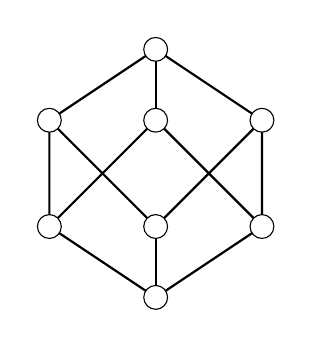
\begin{tikzpicture}[scale=.45]
  \draw[thick] (0,0) -- (-3,2) -- (-3,5) -- (0,7) -- (3,5) -- (3,2) -- (0,0);
  \draw[thick] (3,5) -- (0,2) -- (-3,5);
  \draw[thick] (0,0) -- (0,2);
  \draw[thick] (-3,2) -- (0,5) -- (3,2);
  \draw[thick] (0,5) -- (0,7);
  \node (zero) at (0,0) {\tikz\draw[black,fill=white] (0,0) circle (1ex);};
  \node (1) at (-3,2) {\tikz\draw[black,fill=white] (0,0) circle (1ex);};
  \node (2) at (0,2) {\tikz\draw[black,fill=white] (0,0) circle (1ex);};
  \node (3) at (3,2) {\tikz\draw[black,fill=white] (0,0) circle (1ex);};
  \node (4) at (-3,5) {\tikz\draw[black,fill=white] (0,0) circle (1ex);};
  \node (5) at (0,5) {\tikz\draw[black,fill=white] (0,0) circle (1ex);};
  \node (6) at (3,5) {\tikz\draw[black,fill=white] (0,0) circle (1ex);};
  \node (7) at (0,7) {\tikz\draw[black,fill=white] (0,0) circle (1ex);};
\end{tikzpicture}
\captionof{figure}{Example of a poset.}
%\end{figure}
\end{minipage}
\begin{minipage}{0.01\textwidth}
~
\end{minipage}
\begin{minipage}[b]{0.495\textwidth}
%\begin{figure}[H]
\centering
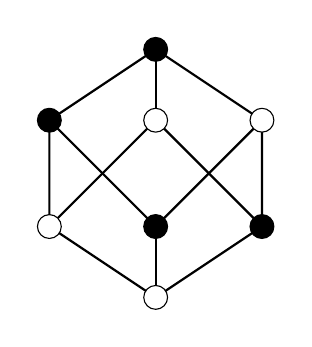
\begin{tikzpicture}[scale=.45]
  \draw[thick] (0,0) -- (-3,2) -- (-3,5) -- (0,7) -- (3,5) -- (3,2) -- (0,0);
  \draw[thick] (3,5) -- (0,2) -- (-3,5);
  \draw[thick] (0,0) -- (0,2);
  \draw[thick] (-3,2) -- (0,5) -- (3,2);
  \draw[thick] (0,5) -- (0,7);
  \node (zero) at (0,0) {\tikz\draw[black,fill=white] (0,0) circle (1ex);};
  \node (1) at (-3,2) {\tikz\draw[black,fill=white] (0,0) circle (1ex);};
  \node (2) at (0,2) {\tikz\draw[black,fill=black] (0,0) circle (1ex);};
  \node (3) at (3,2) {\tikz\draw[black,fill=black] (0,0) circle (1ex);};
  \node (4) at (-3,5) {\tikz\draw[black,fill=black] (0,0) circle (1ex);};
  \node (5) at (0,5) {\tikz\draw[black,fill=white] (0,0) circle (1ex);};
  \node (6) at (3,5) {\tikz\draw[black,fill=white] (0,0) circle (1ex);};
  \node (7) at (0,7) {\tikz\draw[black,fill=black] (0,0) circle (1ex);};
\end{tikzpicture}
\captionof{figure}{Example of a colored poset.}
%\end{figure}
\end{minipage}
\end{ex}
~\\%\newpage
In particular, this thesis focuses on poset games with a specific coloring called chess-coloring.
\\
\begin{minipage}[t]{0.40\textwidth}
\begin{defn}[Chess-Colored Posets]
A \emph{chess-colored poset} is a colored poset such that no element covers an element of the same color. Equivalently we may regard $P=W\cup B$ as a bipartite graph, with white vertices $W$ and black vertices $B$, with the cover relation as an edge relation.
\\
To avoid confusion, we will assume that the least element is colored white when there is only one smallest element.
\end{defn}
\end{minipage}
\begin{minipage}{0.04\textwidth}
~
\end{minipage}
%\begin{figure}[h]
\begin{minipage}[t]{0.55\textwidth}
\begin{ex}{}~
\\
\begin{center}
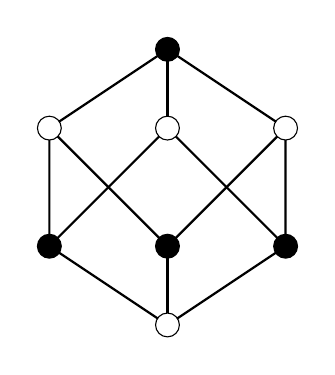
\begin{tikzpicture}[baseline=0.65ex,scale=.5]
  \draw[thick] (0,0) -- (-3,2) -- (-3,5) -- (0,7) -- (3,5) -- (3,2) -- (0,0);
  \draw[thick] (3,5) -- (0,2) -- (-3,5);
  \draw[thick] (0,0) -- (0,2);
  \draw[thick] (-3,2) -- (0,5) -- (3,2);
  \draw[thick] (0,5) -- (0,7);
  \node (zero) at (0,0) {\tikz\draw[black,fill=white] (0,0) circle (1ex);};
  \node (1) at (-3,2) {\tikz\draw[black,fill=black] (0,0) circle (1ex);};
  \node (2) at (0,2) {\tikz\draw[black,fill=black] (0,0) circle (1ex);};
  \node (3) at (3,2) {\tikz\draw[black,fill=black] (0,0) circle (1ex);};
  \node (4) at (-3,5) {\tikz\draw[black,fill=white] (0,0) circle (1ex);};
  \node (5) at (0,5) {\tikz\draw[black,fill=white] (0,0) circle (1ex);};
  \node (6) at (3,5) {\tikz\draw[black,fill=white] (0,0) circle (1ex);};
  \node (7) at (0,7) {\tikz\draw[black,fill=black] (0,0) circle (1ex);};
\end{tikzpicture}
%\caption{Example of a chess-colored poset.}
\captionof{figure}{Example of a chess-colored poset.}
\end{center}
\end{ex}
\end{minipage}
%\end{figure}
%\begin{minipage}{0.05\textwidth}
%~
%\end{minipage}
%\begin{minipage}[b]{0.475\textwidth}
%\centering
%\begin{tikzpicture}[scale=.5]
%  \node (zero) at (0,0) {\tikz\draw[black,fill=white] (0,0) circle (.5ex);};
%  \node (1) at (-3,2) {\tikz\draw[black,fill=black] (0,0) circle (.5ex);};
%  \node (2) at (0,2) {\tikz\draw[black,fill=black] (0,0) circle (.5ex);};
%  \node (3) at (3,2) {\tikz\draw[black,fill=black] (0,0) circle (.5ex);};
%  \node (4) at (-3,5) {\tikz\draw[black,fill=white] (0,0) circle (.5ex);};
%  \node (5) at (0,5) {\tikz\draw[black,fill=white] (0,0) circle (.5ex);};
%  \node (6) at (3,5) {\tikz\draw[black,fill=white] (0,0) circle (.5ex);};
%  \node (7) at (0,7) {\tikz\draw[black,fill=black] (0,0) circle (.5ex);};
%  \draw[thick] (zero) -- (1) -- (4);
%  \draw[thick] (6) -- (2) -- (zero);
%  \draw[thick] (5) -- (7);
%  \draw[thick] (1) -- (5) -- (7);
%  \draw[thick] (zero) -- (3);
%\end{tikzpicture}
%\captionof{figure}{Example of a (chess-colored) tree poset.}
%\end{minipage}
%%\end{figure}
%\\\\
%%\begin{minipage}[b]{0.5\textwidth}
%\begin{defn}[Tree Posets]
%A \emph{tree poset} is a poset that, when regarded as a graph with the cover relations as undirected edges, has no cycles. A forest poset is a poset where all components of the poset (when the poset is regarded as a graph with the cover relations as undirected edges) are tree posets.
%\end{defn}
%%\end{minipage}
%%\begin{minipage}{0.1\textwidth}
%%~
%%\end{minipage}
%%\begin{figure}[h]
%%
\subsubsection{Young Diagrams}
This thesis mainly focuses on an object called \emph{Young diagram}. We will formally define exactly what a Young diagram is in Definition \ref{def:lambda}, but before that we need the following definition:
\begin{defn}
\label{def:lambda}
Let $\lambda=(\lambda_1,\dots,\lambda_k)$ be a weakly decreasing sequence of positive integers, i.e., $\lambda_1\ge \lambda_2\ge\dots\ge \lambda_k$. We say that $\lambda$ partitions $n$, denoted by $\lambda\vdash n$, if $\sum_{i=1}^k\lambda_i =n$.
\end{defn}
%~
\begin{defn}[Young Diagrams%{\cite[p.~155]{hk2002}}
]
A \emph{Young diagram} is a collection of boxes arranged in left-justified rows with a weakly decreasing number of boxes in each row. If the number of boxes is $n$ and $\lambda\vdash n$, we say that $\lambda$ generate a Young diagram with $\lambda_1$ boxes in the first row, $\lambda_2$ boxes in the second row,$\dots$, $\lambda_k$ in the $k$'th row.
Moreover, a Young diagram can always be represented as a poset.
\end{defn}
~\\
This definition is best illustrated with an example. 
\begin{ex}{}
With $\lambda=(7,5,2,2,1)$ we have the Young diagram in Figure \ref{fig:youngex} and the corresponding representation as a poset in Figure \ref{fig:youngposetex}.
\\
%\begin{picex}{}
\begin{minipage}[b]{0.45\textwidth}
%\begin{math}
\centering
\begin{tabular}{ | c | c | c | c | c | c | c |}
\hline
~&~&~&~&~&~&~\\
\hline
~&~&~&~&~\\
\cline{1-5}
~&~\\
\cline{1-2}
~&~\\
\cline{1-2}
~\\
\cline{1-1}
\end{tabular}
%\end{math}
\captionof{figure}{Young diagram generated by $\lambda=(7,5,2,2,1)$.}
\label{fig:youngex}
\end{minipage}
%\begin{center}
%\begin{figure}
%\begin{Young}
 %& & & & & & \cr
 %& & & & \cr
 %& \cr
 %& \cr
 %\cr
%\end{Young}
%\end{figure}
%\end{center}
\begin{minipage}{0.05\textwidth}
~%This Young diagram can also be represented as the following poset:
\end{minipage}
\begin{minipage}[b]{0.50\textwidth}
\centering
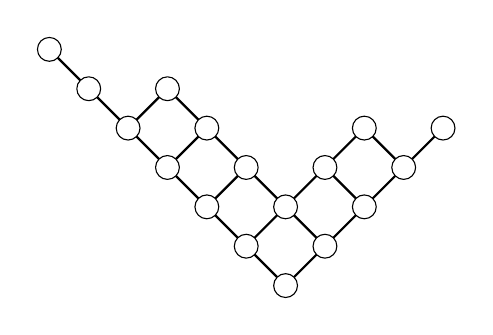
\begin{tikzpicture}[scale=.5]
  \draw[thick] (0,0) -- (-1,1) -- (-2,2) -- (-3,3) -- (-4,4) -- (-5,5) -- (-6,6);
  \draw[thick] (1,1) -- (0,2) -- (-1,3) -- (-2,4) -- (-3,5);
  \draw[thick] (2,2) -- (1,3);
  \draw[thick] (3,3) -- (2,4);
  \draw[thick] (0,0) -- (1,1) -- (2,2) -- (3,3) -- (4,4);
  \draw[thick] (-1,1) -- (0,2) -- (1,3) -- (2,4);
  \draw[thick] (-2,2) -- (-1,3);
  \draw[thick] (-3,3) -- (-2,4);
  \draw[thick] (-4,4) -- (-3,5);
  \node (zero) at (0,0) {\tikz\draw[black,fill=white] (0,0) circle (1ex);};
  \node (1) at (-1,1) {\tikz\draw[black,fill=white] (0,0) circle (1ex);};
  \node (2) at (-2,2) {\tikz\draw[black,fill=white] (0,0) circle (1ex);};
  \node (3) at (-3,3) {\tikz\draw[black,fill=white] (0,0) circle (1ex);};
  \node (4) at (-4,4) {\tikz\draw[black,fill=white] (0,0) circle (1ex);};
  \node (5) at (-5,5) {\tikz\draw[black,fill=white] (0,0) circle (1ex);};
  \node (6) at (-6,6) {\tikz\draw[black,fill=white] (0,0) circle (1ex);};
  \node (7) at (1,1) {\tikz\draw[black,fill=white] (0,0) circle (1ex);};
  \node (8) at (0,2) {\tikz\draw[black,fill=white] (0,0) circle (1ex);};
  \node (9) at (-1,3) {\tikz\draw[black,fill=white] (0,0) circle (1ex);};
  \node (10) at (-2,4) {\tikz\draw[black,fill=white] (0,0) circle (1ex);};
  \node (11) at (-3,5) {\tikz\draw[black,fill=white] (0,0) circle (1ex);};
  \node (12) at (2,2) {\tikz\draw[black,fill=white] (0,0) circle (1ex);};
  \node (13) at (1,3) {\tikz\draw[black,fill=white] (0,0) circle (1ex);};
  \node (14) at (3,3) {\tikz\draw[black,fill=white] (0,0) circle (1ex);};
  \node (15) at (2,4) {\tikz\draw[black,fill=white] (0,0) circle (1ex);};
  \node (16) at (4,4) {\tikz\draw[black,fill=white] (0,0) circle (1ex);};
\end{tikzpicture}
\captionof{figure}{Poset of the Young diagram generated by $\lambda=(7,5,2,2,1)$.}
\label{fig:youngposetex}
\end{minipage}
\end{ex}
In analogy with the previous definitions, a colored Young diagram is a Young diagram where each box has a color of either black or white, and a chess-colored Young diagram is a Young diagram where no adjacent boxes have the same color.
%\\
\begin{ex}{}
With $\lambda=(7,5,2,2,1)$ as before, we have the chess-colored Young diagram and the corresponding chess-colored poset in Figures \ref{fig:chessyoung} and \ref{fig:chessyoungposet} respectively.
\\
%\begin{picex}{}
\begin{minipage}[b]{0.45\textwidth}
%\begin{figure}[H]
\centering
\begin{tabular}{ | c | c | c | c | c | c | c |}
\hline
~&\cellcolor[gray]{0}&~&\cellcolor[gray]{0}&~&\cellcolor[gray]{0}&~\\
\hline
\cellcolor[gray]{0}&~&\cellcolor[gray]{0}&~&\cellcolor[gray]{0}\\
\cline{1-5}
~&\cellcolor[gray]{0}\\
\cline{1-2}
\cellcolor[gray]{0}&~\\
\cline{1-2}
~\\
\cline{1-1}
\end{tabular}
\captionof{figure}{Chess-colored Young diagram generated by $\lambda=(7,5,2,2,1)$.}
\label{fig:chessyoung}
%\end{figure}
\end{minipage}
\begin{minipage}{0.05\textwidth}
~
\end{minipage}
\begin{minipage}[b]{0.5\textwidth}
%\begin{figure}[H]
\centering
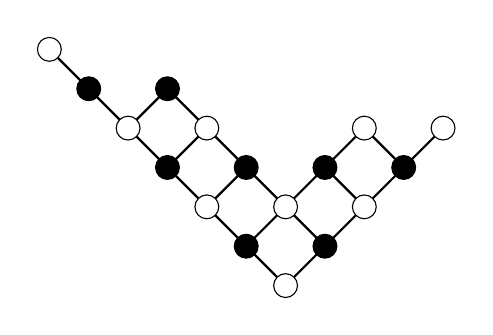
\begin{tikzpicture}[scale=.5]
  \draw[thick] (0,0) -- (-1,1) -- (-2,2) -- (-3,3) -- (-4,4) -- (-5,5) -- (-6,6);
  \draw[thick] (1,1) -- (0,2) -- (-1,3) -- (-2,4) -- (-3,5);
  \draw[thick] (2,2) -- (1,3);
  \draw[thick] (3,3) -- (2,4);
  \draw[thick] (0,0) -- (1,1) -- (2,2) -- (3,3) -- (4,4);
  \draw[thick] (-1,1) -- (0,2) -- (1,3) -- (2,4);
  \draw[thick] (-2,2) -- (-1,3);
  \draw[thick] (-3,3) -- (-2,4);
  \draw[thick] (-4,4) -- (-3,5);
  \node (zero) at (0,0) {\tikz\draw[black,fill=white] (0,0) circle (1ex);};
  \node (1) at (-1,1) {\tikz\draw[black,fill=black] (0,0) circle (1ex);};
  \node (2) at (-2,2) {\tikz\draw[black,fill=white] (0,0) circle (1ex);};
  \node (3) at (-3,3) {\tikz\draw[black,fill=black] (0,0) circle (1ex);};
  \node (4) at (-4,4) {\tikz\draw[black,fill=white] (0,0) circle (1ex);};
  \node (5) at (-5,5) {\tikz\draw[black,fill=black] (0,0) circle (1ex);};
  \node (6) at (-6,6) {\tikz\draw[black,fill=white] (0,0) circle (1ex);};
  \node (7) at (1,1) {\tikz\draw[black,fill=black] (0,0) circle (1ex);};
  \node (8) at (0,2) {\tikz\draw[black,fill=white] (0,0) circle (1ex);};
  \node (9) at (-1,3) {\tikz\draw[black,fill=black] (0,0) circle (1ex);};
  \node (10) at (-2,4) {\tikz\draw[black,fill=white] (0,0) circle (1ex);};
  \node (11) at (-3,5) {\tikz\draw[black,fill=black] (0,0) circle (1ex);};
  \node (12) at (2,2) {\tikz\draw[black,fill=white] (0,0) circle (1ex);};
  \node (13) at (1,3) {\tikz\draw[black,fill=black] (0,0) circle (1ex);};
  \node (14) at (3,3) {\tikz\draw[black,fill=black] (0,0) circle (1ex);};
  \node (15) at (2,4) {\tikz\draw[black,fill=white] (0,0) circle (1ex);};
  \node (16) at (4,4) {\tikz\draw[black,fill=white] (0,0) circle (1ex);};
\end{tikzpicture}
\captionof{figure}{Chess-colored poset of the Young diagram in figure \ref{fig:chessyoung}.}
\label{fig:chessyoungposet}
%\end{figure}
\end{minipage}
\end{ex}


\subsection{Combinatorial Game Theory}
This thesis deals with combinatorial game theory, an area which studies sequential games with perfect information, that is, games where the players play in turns and where they have complete knowledge of the game, i.e., know all possible game options for all players. 
\\
In particular, the thesis will focus on two-player partizan combinatorial games, in which the game options of the two players can be different. Furthermore, we call the two players Left and Right (or White and Black or Blue and Red).
\\
In general, a combinatorial game has \emph{positions}, and at any given position every player has a set of \emph{options} of moving to a new position. Under normal play convention a player loses if they have no options available at their turn to move.
%\\
\begin{defn}[Partizan Game Position{\cite[p.~71]{onag}}]
A position in a partizan game is defined by its left and right options, and we denote it by $G=\{L|R\}$, where $L$ and $R$ are the sets of left and right options respectively. 
\end{defn}
~\\
Since we will be using the notation used by Conway\cite{onag}, the notation above will not always be used, and we will instead often abuse it by writing $G=\{G_1,G_2,G_3|H_1,H_2\}$ as short for $G=\left\{\{G_1,G_2,G_3\}|\{H_1,H_2\}\right\}$, and in the general case $G=\{G^L|G^R\}$.
\\
Following this we will introduce some notation for the games depending on the winner and who starts.
%\\
\begin{defn}[Value Notation{\cite[p.~73]{onag}}]
\label{def:value}
~
\begin{itemize}
\item $G>0$ ($G$ is \emph{positive}) if there is a winning strategy for Left.
\item $G<0$ ($G$ is \emph{negative}) if there is a winning strategy for Right.
\item $G=0$ ($G$ is \emph{zero}) if there is a winning strategy for the second player to move.
\item $G\parallel0$ ($G$ is \emph{fuzzy} to zero) if there is a winning strategy for first player move.
\end{itemize}
\end{defn}
~\\
This notation is easy to understand with help of some examples.
%\\
\begin{ex}{}
Consider the simplest possible game, the game with no options for either player, i.e., $G_1=\{|\}$. We obviously have $G_1=0$, since the first player has no options to play and therefore loses. This game is denoted by $0:=\{|\}$.
\\
Now consider the game where Left has the option to move to $0$, but Right still has no options, i.e., $G_2=\{0|\}$. Here we have that $G_2>0$ since either Left starts and moves to $0$, and then Right has no option and loses, or Right starts and has no options and therefore loses, i.e., Left has a winning strategy. This game is denoted by $1:=\{0|\}$. Similarly we have that the game $-1<0$ where $-1$ is defined as $-1:=\{|0\}$.
\\
Finally, consider the game where both players have the option to move to $0$, i.e., $G_3=\{0|0\}$. We now have $G_3\parallel0$ since both players have the option to move to $0$, where the second player then will lose. This game is denoted as $*:=\{0|0\}$.
\end{ex}
%\newpage
~\\
The value notation of Definition \ref{def:value} can be combined and extended in the following way.
\begin{defn}[Extended Value Notation{\cite[p.~73]{onag}}]
\label{def:extvalue}~
\begin{itemize}
\item If $G\ge0$, then Left always wins if Left is the second player to move.
\item If $G\le0$, then Right always wins if Right is the player second to move.
\item If $G\rhd0$, then Left always wins if Left is the first player to move.
\item If $G\lhd0$, then Right always wins if Right is the first player to move.
\end{itemize}
\end{defn}
~\\
In addition to the value notations, it is also possible to add and subtract games.
\begin{defn}[Addition and Negation{\cite[p.~73]{onag}}]
\begin{align*}
G+H&=\left\{G^L+H,G+H^L\middle|G^R+H,G+H^R\right\}\\
-G&=\left\{-G^R\middle|-G^L\right\}
\end{align*}
\end{defn}
~\\
Informally, we can note that addition of two games is the same as playing in both games at the same time, and the negation of a game is the game with reversed roles of Left and Right. Combining these, it is possible to subtract games as $G-H=G+(-H)$. 
\\
Using this, we define the following relations between games:
\begin{defn}[Game Relations{\cite[p.~78]{onag}}]
~
\begin{itemize}
\item $G>H$ iff $G-H>0$.
\item $G<H$ iff $G-H<0$.
\item $G=H$ iff $G-H=0$.
\item $G\parallel H$ iff $G-H\parallel0$.
\end{itemize}
\end{defn}
~\\
Using these relations, which can be combined and extended as the extended notation of Definition \ref{def:extvalue}, we can define what a \emph{dominated} option is.
\begin{defn}[Dominated Options{\cite[p.~110]{onag}}]
\label{def:dominate}
For a game we say that a left option $G^{L_1}$ is dominated by another left option option $G^{L_0}$ if $G^{L_1}\le G^{L_0}$. Similarly, a right option $G^{R_1}$ is dominated by another right option $G^{R_0}$ if $G^{R_1}\ge G^{R_0}$.
\end{defn}
~\\
In fact, an important property of a game is that you always can remove any dominated options{\cite[p.~110]{onag}}.
\begin{thm}
\label{thm:domopt}
Let $G=\left\{G^{L_0},G^{L_1},\dots|G^{R_0},G^{R_1}\dots,\right\}$. 
\begin{itemize}
\item If $G^{L_0}\le G^{L_1}$, then $G=G'$, where $G'=\left\{G^{L_1},\dots|G^{R_0},G^{R_1}\dots,\right\}$.
\item If $G^{R_0}\ge G^{R_1}$, then $G=G''$, where $G''=\left\{G^{L_0},G^{L_1},\dots|G^{R_1}\dots,\right\}$.
\end{itemize}
\end{thm}
~\\
A significant class of games are the \emph{short} games.
\begin{defn}[Short Games{\cite[p.~3]{lip}\cite[p.97]{onag}}]
A game G is short if only a finite number of positions can be reached and a position may never be repeated.
\end{defn}
~\\
Moreover, every short game $G$ has a unique simplest form. This is called $G$'s canonical form{\cite[p.~78]{lip}}. It is possible to reduce any short game to its canonical form by just removing dominated and \emph{reversible} options{\cite[p.~111]{onag}}.
\\\\
A methodology that is extremely useful when proving properties of games is \emph{Conway induction}.
\begin{thm}[Conway Induction{\cite[p.~5]{onag}}]
\label{thm:conind}
Let $P$ be a property which games might have, such that any game $G$ has property $P$ whenever all left and right options of $G$ have this property. Then every game has property $P$.
\end{thm}
~\\
The methodology using Conway induction makes it possible to prove that a game has a property by assuming that all its options have this property, and from this proving that the game itself has it. This methodology is using that the definitions of games are inductive.
\subsubsection{Numbers}
\label{section:numbers}
Another important property and concept in combinatorial games is that of numbers, which is a class of games with some special characteristics. 
%\\
\begin{defn}[Numbers{\cite[p.~91]{lip}}]
A number is any game $x$ such that all $x^L<x<x^R$ and $x^L$ and $x^R$ are numbers.
For short games, we can, equivalently, for $j>0$ and $m$ odd, define a number as
\begin{equation}
\frac{m}{2^j}=\left\{\frac{m-1}{2^j}\Bigg|\frac{m+1}{2^j}\right\}.
\label{eq:number}
\end{equation}
\label{def:number}
\end{defn}
~\\
It should also be noted that all games are not numbers. For $*=\{0|0\}$ we have $G^L=0=G^R$, and hence $G^L\not<G^R$, i.e., $*$ is not a number.
\\
Equation (\ref{eq:number}) can be generalized to recognize when $G$ is a number even if it is not in canonical form. For this, we need to define what the \emph{simplest number} is.
%\\
\begin{defn}[Simplest Number{\cite[p.~93]{lip}}]
\label{def:simpnum}
For $x^L<x^R$, the simplest number $x$ between $x^L$ and $x^R$ is given by the following:
\begin{itemize}
\item If there are integer(s) $n$ such that $x^L<n<x^R$, $x$ is the one that is smallest in absolute value.
\item Otherwise, $x$ is the number of the form $\frac{i}{2^j}$ between $x^L$ and $x^R$ for which $j$ is minimal.
\end{itemize}
\end{defn}
%~
\begin{thm}[Numbers{\cite[p.~93]{lip}}]
\label{thm:number}
If all options of a game $G$ are numbers and all $G^L<G^R$, then $G$ is the simplest number $x$ satisfying $G^L<x<G^R$. 
\end{thm}
~\\
This, together with Definition \ref{def:dominate} and Theorem \ref{thm:domopt}, yields that a game that is equal to a number is equal to the game consisting of only its greatest left options and smallest right options, i.e., 
$G\equiv\left\{G^{L_0},G^{L_1},\dots|G^{R_0},G^{R_1}\dots,\right\}=\left\{G^{L_0}|G^{R_0}\right\}\equiv G'$ if $G^{L_0}\ge G^{L_i}$ and $G^{R_0}\le G^{R_j}$ for $i,j>0$. 
\\
It should also be noted that equation (\ref{eq:number}) is a number for integers $j>0$ and $m$, regardless if $m$ is odd or not.

\subsubsection{Hackenbush}
A game with properties similar to the ones studied in this thesis is \emph{Blue-Red Hackenbush}. Hackenbush is a partizan two-player game that may be played on any configuration of colored line segments connected to one another by their endpoints and to a "ground" line. In the Blue-Red Hackenbush, the line segments are colored either blue or red. It is played by, in turns, removing a line segment of your color, by which all segments that are unconnected to the ground vanishes, until a player has no move left.
\begin{ex}{}
\label{ex:hack}
An example of a game of Blue-Red Hackenbush and gameplay on that game.
\begin{figure}[H]
\centering
{\Large
$
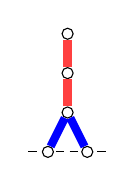
\begin{tikzpicture}[baseline=-0.65ex,scale=0.5]
    \draw[densely dashed] (-1,-1) -- (1,-1);
    \node[hackennode] (middle) at ( 0,   0) {};
    \node[hackennode] (left)   at (-0.5,-1) {};
    \node[hackennode] (right)  at ( 0.5,-1) {};
    \node[hackennode] (top)    at ( 0,   1) {};
    \node[hackennode] (top2)   at ( 0,   2) {};

    \draw[hackenline,blue]
        (left) -- (middle) -- (right);
    \draw[hackenline,red!75]
        (middle) -- (top);
    \draw[hackenline,red!75]
        (top) -- (top2);
\end{tikzpicture}
=
\left\{
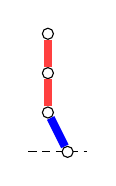
\begin{tikzpicture}[baseline=-0.65ex,scale=0.5]
    \draw[densely dashed] (-0.5,-1) -- (1,-1);
    \node[hackennode] (middle) at ( 0,   0) {};
    \node[hackennode] (right)  at ( 0.5,-1) {};
    \node[hackennode] (top)    at ( 0,   1) {};
    \node[hackennode] (top2)   at ( 0,   2) {};

    \draw[hackenline,blue]
        (middle) -- (right);
    \draw[hackenline,red!75]
        (middle) -- (top);
    \draw[hackenline,red!75]
        (top) -- (top2);
\end{tikzpicture}
\tikz[baseline=-0.65ex,scale=0.5] \node[inner sep=0] at (0,-1) {,\,};
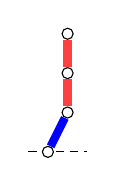
\begin{tikzpicture}[baseline=-0.65ex,scale=0.5]
    \draw[densely dashed] (-1,-1) -- (0.5,-1);
    \node[hackennode] (middle) at ( 0,   0) {};
    \node[hackennode] (left)   at (-0.5,-1) {};
    \node[hackennode] (top)    at ( 0,   1) {};
    \node[hackennode] (top2)   at ( 0,   2) {};

    \draw[hackenline,blue]
        (middle) -- (left);
    \draw[hackenline,red!75]
        (middle) -- (top);
    \draw[hackenline,red!75]
        (top) -- (top2);
\end{tikzpicture}
\middle|
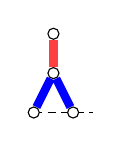
\begin{tikzpicture}[baseline=-0.65ex,scale=0.5]
    \draw[densely dashed] (-0.5,-1) -- (1,-1);
    \node[hackennode] (middle) at ( 0,   0) {};
    \node[hackennode] (left)   at (-0.5,-1) {};
    \node[hackennode] (right)  at ( 0.5,-1) {};
    \node[hackennode] (top)    at ( 0,   1) {};

    \draw[hackenline,blue]
        (left) -- (middle) -- (right);
    \draw[hackenline,red!75]
        (middle) -- (top);
\end{tikzpicture}
\tikz[baseline=-0.65ex,scale=0.5] \node[inner sep=0] at (0,-1) {,\,};
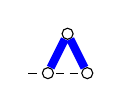
\begin{tikzpicture}[baseline=-0.65ex,scale=0.5]
    \draw[densely dashed] (-1,-1) -- (0.5,-1);
    \node[hackennode] (middle) at ( 0,   0) {};
    \node[hackennode] (left)   at (-0.5,-1) {};
    \node[hackennode] (right)  at ( 0.5,-1) {};

    \draw[hackenline,blue]
        (left) -- (middle) -- (right);
\end{tikzpicture}
\right\}
$
}% End group with \Large
\caption{A simple game of Blue-Red Hackenbush.}
\label{fig:hackenbush}
\end{figure}
\begin{figure}[H]
{\Large
\[
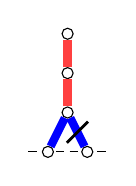
\begin{tikzpicture}[baseline=-0.65ex,scale=0.5]
    \draw[densely dashed] (-1,-1) -- (1,-1);
    \node[hackennode] (middle) at ( 0,   0) {};
    \node[hackennode] (left)   at (-0.5,-1) {};
    \node[hackennode] (right)  at ( 0.5,-1) {};
    \node[hackennode] (top)    at ( 0,   1) {};
    \node[hackennode] (top2)   at ( 0,   2) {};

    \draw[hackenline,blue]
        (left) -- (middle) -- node[strike out,draw=black,line width=1,-]{}(right);
    \draw[hackenline,red!75]
        (middle) -- (top);
    \draw[hackenline,red!75]
        (top) -- (top2);
\end{tikzpicture}
\overset{L}{\longrightarrow}
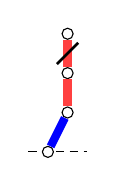
\begin{tikzpicture}[baseline=-0.65ex,scale=0.5]
    \draw[densely dashed] (-1,-1) -- (0.5,-1);
    \node[hackennode] (middle) at ( 0,   0) {};
    \node[hackennode] (left)   at (-0.5,-1) {};
    \node[hackennode] (top)    at ( 0,   1) {};
    \node[hackennode] (top2)   at ( 0,   2) {};

    \draw[hackenline,blue]
        (middle) -- (left);
    \draw[hackenline,red!75]
        (middle) -- (top);
    \draw[hackenline,red!75]
        (top) -- node[strike out,draw=black,line width=1,-]{}(top2);
\end{tikzpicture}
\overset{R}{\longrightarrow}
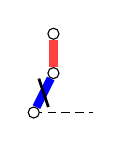
\begin{tikzpicture}[baseline=-0.65ex,scale=0.5]
    \draw[densely dashed] (-0.5,-1) -- (1,-1);
    \node[hackennode] (middle) at ( 0,   0) {};
    \node[hackennode] (left)   at (-0.5,-1) {};
    \node[hackennode] (top)    at ( 0,   1) {};

    \draw[hackenline,blue]
        (middle) -- node [sloped,strike out,draw=black,line width=1,-]{}(left);
    \draw[hackenline,red!75]
        (middle) -- (top);
\end{tikzpicture}
\overset{L}{\longrightarrow}
\begin{tikzpicture}[baseline=-0.65ex,scale=0.5]
    \draw[densely dashed] (-1,-1) -- (0.5,-1);
\end{tikzpicture}
\]
}% End group with \Large
\caption{Example of gameplay on the Blue-Red Hackenbush in Figure \ref{fig:hackenbush} where Left player wins.}
\end{figure}
\end{ex}
It is known that every game of Blue-Red Hackenbush is a surreal number, and in particular, any \emph{finite} game of Blue-Red Hackenbush is a dyadic rational number, i.e., on the form $\frac{m}{2^j}$ where $m$ and $j>0$ are integers.
\subsubsection{Chomp}
\label{section:chomp}
\begin{minipage}[b]{0.5\textwidth}
Another game closely related to that of this thesis is the game of \emph{Chomp}. Chomp is a impartial two-player game with the usual starting position consisting of a rectangle (possibly infinite) with one poison square in the lower-left corner. A move in Chomp is to choose a square and remove this and all other squares above or to the right of it, and a player loses if they has to choose the poison square.
\end{minipage}
\begin{minipage}{0.05\textwidth}
~
\end{minipage}
\begin{minipage}[b]{0.45\textwidth}
%\begin{figure}[H]
\centering
\begin{tabular}{ | c | c | c | c | c |}
\hline
~&~&~&~&~\\
\hline
~&~&~&~&~\\
\hline
~&~&~&~&~\\
\hline
~&~&~&~&~\\
\hline
~&~&~&~&~\\
\hline
~&~&~&~&~\\
\hline
\cellcolor{red}&~&~&~&~\\
\hline
\end{tabular}
\captionof{figure}{Example of a starting position of a game of Chomp.}
\label{fig:chompstart}
%\end{figure}
\end{minipage}
\begin{ex}{}
\label{ex:chompgame}
An example of gameplay on a game of Chomp with starting position as in Figure \ref{fig:chompstart}.
\begin{figure}[H]
\centering
$
\begin{tabular}{ | c | c | c | c | c |}
\hhline{-----}
~&~&~&\cellcolor[gray]{0.8}&\cellcolor[gray]{0.8}\\
\hhline{-----}
~&~&~&\cellcolor[gray]{0.8}&\cellcolor[gray]{0.8}\\
\hhline{-----}
~&~&~&\cellcolor[gray]{0.8}&\cellcolor[gray]{0.8}\\
\hhline{-----}
~&~&~&\cellcolor[gray]{0.8}&\cellcolor[gray]{0.8}\\
\hhline{-----}
~&~&~&\cellcolor[gray]{0.8}&\cellcolor[gray]{0.8}\\
\hhline{-----}
~&~&~&\cellcolor[gray]{0.6}&\cellcolor[gray]{0.8}\\
\hhline{-----}
\cellcolor{red}&~&~&~&~\\
\hhline{-----}
\end{tabular}
\overset{L}{\longrightarrow}
\begin{tabular}{ | c | c | c | c | c |}
\hhline{---~~}
\cellcolor[gray]{0.8}&\cellcolor[gray]{0.8}&\cellcolor[gray]{0.8}\\
\hhline{---~~}
\cellcolor[gray]{0.8}&\cellcolor[gray]{0.8}&\cellcolor[gray]{0.8}\\
\hhline{---~~}
\cellcolor[gray]{0.8}&\cellcolor[gray]{0.8}&\cellcolor[gray]{0.8}\\
\hhline{---~~}
\cellcolor[gray]{0.8}&\cellcolor[gray]{0.8}&\cellcolor[gray]{0.8}\\
\hhline{---~~}
\cellcolor[gray]{0.6}&\cellcolor[gray]{0.8}&\cellcolor[gray]{0.8}\\
\hhline{---~~}
~&~&~\\
\hhline{-----}
\cellcolor{red}&~&~&~&~\\
\hhline{-----}
\end{tabular}
\overset{R}{\longrightarrow}
\begin{tabular}{ | c | c | c | c | c |}
\hhline{---~~}
~&\cellcolor[gray]{0.8}&\cellcolor[gray]{0.8}\\
\hhline{-----}
\cellcolor{red}&\cellcolor[gray]{0.6}&\cellcolor[gray]{0.8}&\cellcolor[gray]{0.8}&\cellcolor[gray]{0.8}\\
\hhline{-----}
\end{tabular}
\overset{L}{\longrightarrow}
\begin{tabular}{ | c |}
\hhline{-}
\cellcolor[gray]{0.6}\\
\hhline{-}
\cellcolor{red}\\
\hhline{-}
\end{tabular}
\overset{R}{\longrightarrow}
\begin{tabular}{ | c |}
\hline
\cellcolor{red}\\
\hline
\end{tabular}
$
\captionof{figure}{Example of gameplay in the game of Chomp with starting position as in Figure \ref{fig:chompstart} where Right player wins.}
\end{figure}
\end{ex}
% sparse coding, Discriminative vs Generative, Discriminative Disaggregation Sparse Coding, Non-Negative Sparse Coding
\newpage
\section{Problem Definition}
%• Problem definition: What is demanded from the solution? What is the aim of the study?
%Useful simplifications?
%• Problem definition: What is demanded from the solution? What is the aim of the study?
%Useful simplifications?
In this section we describe what is required of the solution and what this thesis aims at achieving as well as some useful simplifications made for this thesis.


Kotler et. al. \cite{DDSC} train the DDSC algorithm with weeks sampled across two years of data as to generalize the training. This thesis aims at reimplementing the algorithm and investigating the possibility of training with less data but taking the advantage of the temporal correlation between years as to further extend the algorithm by pre-processing the data better, by training the algorithm for the same timeperiod across two years instead of randomly.

\subsection{Solution}
%• Solution/Design: How is it to be done? Will it give the expected performance? What
%limitations can be foreseen from theory?

\begin{enumerate}
	\item{Retrieve similar data}
	\item{Pre-process}
	\item{Implementation}
	\item{Tweak algorithm using temporal difference}
\end{enumerate}

The first problem to address is to retrieve valuable and similar data mostly found via githubs \href{https://github.com/caesar0301/awesome-public-datasets}{Awesome-public-datasets} \cite{awesome}. Once the data has been decided on we pre-process and implement the algorithm, where the algorithm itself could pose a challenge as there is no explicit formulation stated in the paper \cite{DDSC}, nor any source code available. This thesis aims at reproducing the results, by focusing on exploiting the data at hand. The method relies substansually on the data, which could prove to produce very different results. The implementation is limited by the amount of computational power that is available as it run by standard student-laptop. This is reflected on the choice of training set and as well as the choice of number of basis for the algorithms (this is preferably higher in dimension than the dimensionality of the data).
%• Solution/Design: How is it to be done? Will it give the expected performance? What
%limitations can be foreseen from theory?

\newpage
% Method/Fabrication/Experimental setup
\section{Fabrication}
\label{sec:fab}
% - Block coordinate update, Pre-processing, 
This section accounts for the dataset used and the data pre-processing assumptions made for usability, we also visualize the datasets used. In section \ref{sec:ddsc}, we make a complete outline of the algorithm which is the basis for this thesis. Lastly, in section \ref{sec:implementation}, we review what has been implemented in detail and what tools have been.


\subsection{Dataset}

In this paper, the Pecan Street data \cite{pecan} has been solely used. The reason is that most of the current datasets include as much detail, but lack a vast number of houses, which is needed in order for a deep learning to train itself.

\subsection{Data pre-processing}
\label{sec:prep}
If there is much irrelevant and redundant information present or noisy and unreliable data, then knowledge discovery during the training phase is more difficult. Data preparation and filtering steps have taken considerable amount of processing time. The process has included cleaning, normalization, transformation of the dataset, where the end product have been the final training set.

% - different approaches to the problem
The data that has been chosen for creating the training and testing set have been from the year 2014 and 2015. The raw data contain more than 8 billion readings from different appliances in 689 houses. However the problem with most data is incompleteness. The appliances that have been taken into consideration have been; air, furnace, dishwasher, refrigerator and the summed values of the other appliances called miscellaneous category, for more detail visit \href{http://www.pecanstreet.org/}{Pecan Street Inc}. These appliances were chosen due to the lack of information, investigating the dataset revealed that almost 80\% of the values were not present for most monitored appliances. Out of the chosen appliances, a house was taken into account if it had missing values of more than one appliance for each hour. 

For treating missing values we assuming that appliances run as a constant fashion, meaning that we interpolate the nearest value from the previous reading to complete the dataset. Below we find energy readings of the whole-home usage of electricity in the dataset.

\begin{figure}[H]
	\centering
	\includegraphics[scale=0.30]{./figures/houseuse}
	\caption{Training households, 2014}
	\label{fig:houseuse}
\end{figure}

As seen from the figure \ref{fig:houseuse}, some houses end up using almost 10 times more elecricity than the average household. These households have an impact to focus less on the more generalized households. Presumably these households are not of interest for Greenely or the generalized result in which we would want to classify. Here the assumption has been that these households are more of industrial size, although not nearly enough power consumption to be compared to, but acting more of a reference for which households have been investigated.

\begin{figure}[H]
	\centering
	\begin{minipage}{.5\textwidth}
		\centering
		\includegraphics[scale=0.19]{./figures/weekendhouseuse}
		%\label{fig:test6}
	\end{minipage}%
	\begin{minipage}{.5\textwidth}
		\centering
		\includegraphics[scale=0.19]{./figures/weekdayshouseuse}
		%\label{fig:test5}
	\end{minipage}
	\caption{This figure shows two plots representing the weekday and weekend datasets. The datasets are compressed of a whole year of weekdays and weekends respectively. The left plot have values for all the hours of the weekends for a year 2496 hours. The right plot consists of hourly readings of 6240 hours.}
	\label{fig:weekend_day}
\end{figure}

From the figure above \ref{fig:weekend_day}, we can see that the left plot which has the weekends, consists of peaks of consumption. In comparison with the right plot, where we have a more consistent behaviour of the household consumption. However, we note that energy consumption show that it is not significant enough to take into consideration. We conclude that the algorithm could find better shapes within the data when the dataset has been split, however there will probably be no seen affect from the energy consumption.

\begin{figure}[H]
	\centering
	\includegraphics[scale=0.30]{./figures/weekconsump}
	\caption{A week of the consumption data for the appliances and whole-home usage}
	\label{fig:weekconsump}
\end{figure}

The figure shows consumption of the considered appliances. Pecan Street Inc's dataset is a great source of energy consumption data, however they have made a choice of registering average consumption of the particular appliance during that interval, with the aim that; if a refrigerator has been consuming one kilowatt per minute for 10 min and then gets turned off, it will be represented as $\frac{1}{10}$ instead of $\frac{1}{60}$, which could make the observation-based method flawed, as the assumption of precise measurements is the basis of the algorithm that Kotler et. al. presented \cite{DDSC}. 

\begin{figure}[H]
	\centering
		\includegraphics[scale=0.30]{./figures/new_histusage}
		\caption{Histogram of the household usage.}
		\label{fig:histuseage}
\end{figure}

The histogram in figure \ref{fig:histuseage} is presented to show that the usual consumption is substantially around the values 0.2 to 0.8 kW per hour. This is what Energy Information Administration \href{http://www.eia.gov/tools/faqs/faq.cfm?id=97&t=3}{EIA} presented in 2013 \cite{eia}, where they present the average consumption of an American household to 10,908 kilowatthours (kWh) which in turn corresponds to:

\begin{equation*}
	10.908 \textbf{kWh} / (24\times365) \textbf{h} = 1.245205479 \textbf{kW}
\end{equation*}

The average consumption for the Pecan Street households is 1.2244009446607182 \textbf{kW}, in the regard of average consumption the dataset can be seen as a good representation for a general household within the United States. Interesting to note is that the data can be fitted to a Weibull distribution, which has been used for providing dummy data.

\newpage
% --
\subsection{Discriminative Disaggregation via Sparse Coding}
\label{sec:ddsc}
This approach was presented in 2011 by J. Kolter MIT and Batr, Y.Nh from Stanford in \cite{DDSC}. It is based on improvements of single-channel source separation and enable a sparse coding algorithm to learn a model of each device's power consumption over a typical week. These learned models are then combined to predict the power consumption of different devices in previously unseen homes, using only their aggregate signal. Typically these algorithms have been used in audio signal separation, which usually has high temporal resolution (precision of measurement w.r.t. time) in contrast to low-resolution energy disaggregation; which impose new challenges within the field. Their algorithm shows an improvement of discriminatively training sparse coding dictionaries for disaggregation tasks. More specifically, they formulate the task of maximizing disaggregation as a structured prediction problem. 

The sparse coding approach to source separation, which forms for the basis for disaggregation, is to train separate models for each individual class $\mathbf{X}_i \in \mathbb{R}^{T\times m}$, where $T$ is the number of samples (hours in the given timeperiod) and $m$ is the number of features (households included) then use these models to separate an aggregate signal. Formally, sparse coding; models the $i$th data matrix using the approximation $\mathbf{X}_i \approx \mathbf{B}_i\mathbf{A}_i$ where the columns of $\mathbf{B}_i \in \mathbb{R}^{T \times n}$ contain a set of $n$ basis functions, also called the dictionary, and the columns of $\mathbf{A}_i \in \mathbb{R}^{n \times m}$ contain the activations of these basis functions, see section \ref{sec:scnn} for more detail. The data input is describe below:

\begin{itemize}
	\item{We define one class (e.g. heater) $\mathbf{X}_i \leftarrow 1,\dots,
		k$}
	\item{Where $\mathbf{X}_i \in \mathbb{R}^{T \times m}$, ex: week $T=24\times7=168$ of $m$ houses}
	\item{\textbf{One} aggregated household $\bar{\mathbf{X}} \leftarrow \sum_{i:k} \mathbf{X}_i$}
	\item{Assuming we have individual energy readings $\mathbf{X}_1,\dots,\mathbf{X}_k$}
	\item{Sparse encode $\mathbf{A},\mathbf{B}$ such that $(n \gg m,T)$}
	\item{Goal: test with new data $\bar{\mathbf{X}}'$ to components
		$\mathbf{X}_1',\dots,\mathbf{X}_k'$}
\end{itemize}

Sparse Coding additionally imposes the constraint that the activations $\mathbf{A}_i$ be sparse, i.e., that they contain mostly zero entries. This allows for learning \textit{overcomplete} sets of representations of the data (more basis functions than the dimensionality of the data, $n \gg m,T$). This makes sparse coding interesting for the field of energy disaggregation since the input data (energy consumption) is inherently positive. They also impose that the activations and dictionaries (bases) be non-negative, presented by \cite{hoyer} as non-negative sparse coding, see section \ref{sec:nnsc} for more detail. The non-negative sparse coding objective

\begin{equation}
\min_{\mathbf{A} \geq 0} \norm{\mathbf{X}_i - \mathbf{B}_i\mathbf{A}}_F^2 + \lambda \sum_{p,q} \mathbf{A}_{pq} \quad \text{subject to} \quad \norm{\mathbf{b}_i^{(j)}}_2 \leq 1, j=1,\dots,n
\end{equation}

where $\mathbf{X}_i,\mathbf{A}_i$ and $\mathbf{B}_i$ are defined as above, while $\lambda \in \mathbb{R}_+$ is a regularization parameter and norms defined as in beginning of section 2 \ref{sec:theoretical}. The sparse coding optimization problem is convex for each optimization-variable whilst holding the other variable fixed. The most common technique is to alternate between minimizing the objective over $\mathbf{A}_i$ and $\mathbf{B}_i$ \cite{DDSC}.

When the representations have been trained for each of the classes (appliances), we concatenated the bases to form a single joint set of basis functions and solve a disaggregation for a new aggregate signal $\bar{\mathbf{X}} \in \mathbb{R}^{T\times m'}$ using the procedure presented below. 

\begin{equation}
\label{eq:f}
\begin{aligned}
\hat{\mathbf{A}}_{1:k}  & = \arg \! \min_{\mathbf{A_{1:k}} \geq 0} \norm{\bar{\mathbf{X}}-\left[\mathbf{B}_1 \cdots \mathbf{B}_k\right]  
		\begin{bmatrix}
		\mathbf{A}_1 \\
		\vdots \\
		\mathbf{A}_k
		 \end{bmatrix}
	}_F^2 + \lambda \sum_{i,p,q}(\mathbf{A}_i)_{pq} \\
 & \vcentcolon= \arg \! \min_{\mathbf{A_{1:k}} \geq 0} F(\bar{\mathbf{X}},\mathbf{B}_{1:k},\mathbf{A}_{1:k})
\end{aligned}
\end{equation}

where $\mathbf{A}_{1:k}$ is denoted as $[\mathbf{A}_1,\dots,\mathbf{A}_k]$ and we abbreviate the optimization objective as $F(\bar{\mathbf{X}},\mathbf{B}_{1:k},\mathbf{A}_{1:k})$. We then predict the $i$th component of the signal to be 

\begin{equation}
\hat{\mathbf{X}}_i = \mathbf{B}_i \hat{\mathbf{A}_i}.
\end{equation}

The intuition is that if $\mathbf{B}_i$ is trained to reconstruct the $i$th class with small activation, then it should better represent the $i$th portion of the aggregate signal than all other bases $\mathbf{B}_j$ for $j\neq i$. Henceforth they construct a way of evaluating the quality of the resulting disaggregation (\textit{disaggregation error})

\begin{equation}
\label{eq:diserr}
E(\mathbf{X}_{1:k},\mathbf{B}_{1:k}) \vcentcolon= \sum_{i=1}^k \frac{1}{2} \norm{\mathbf{X}_i - \mathbf{B}_i \hat{\mathbf{A}}_i}_F^2 \ \text{s.t.} \ \hat{\mathbf{A}}_{1:k} = \arg \! \min_{\mathbf{A_{1:k}} \geq 0} F\left( \sum_{i=1}^k \mathbf{X}_i,\mathbf{B}_{1:k},\mathbf{A}_{1:k} \right),
\end{equation}

which quantifies the reconstruction process for each individual class when using the activations obtained only via the aggregated signal.

\subsubsection{Structured prediction for Discriminative Disaggregation Sparse Coding}

One of the issues that Andrew Ng and J.Zico Kotler point out, using Sparse Coding, the training is solely done for each appliance at hand when the whole-home consumption from consumers have a large variance, as can be seen in figure \ref{fig:houseuse}. The method revolves around training each individual class to produce a small disaggregation error. It is furthermore hard to optimize the disaggreagtion error direcly over the basis $\mathbf{B}_{1:k}$, ignoring the dependance of $\hat{\mathbf{A}}_{1:k}$ on $\mathbf{B}_{1:k}$, resolving for the activations  $\hat{\mathbf{A}}_{1:k}$ ; thus ignoring the dependance of $\hat{\mathbf{A}}_{1:k}$ on $\mathbf{B}_{1:k}$, which loses much of the problem's structure and this approach performs very poorly in practice.

In their paper they define an augmented regularized disaggregation error objective
\begin{equation}
\label{eq:regerror}
\begin{aligned}
\tilde{E}_{reg}(\mathbf{X}_{1:k},\mathbf{B}_{1:k},\tilde{\mathbf{B}}_{1:k})  & \vcentcolon=  \sum_{i=1}^k \left( \frac{1}{2} \norm{\bar{\mathbf{X}}-\mathbf{B}_i  \hat{\mathbf{A}}_i}_F^2 + \lambda \sum_{i,p,q}(\hat{\mathbf{A}}_i)_{pq} \right) \\
& \text{subject to } \hat{\mathbf{A}}_{1:k} = \arg \! \min_{\mathbf{A_{1:k}} \geq 0} F\left(\sum_{i=1}^k \mathbf{X}_i,\tilde{\mathbf{B}}_{1:k},\mathbf{A}_{1:k}\right),
\end{aligned}
\end{equation}

where the $\mathbb{B}_{1:k}$ bases (referred to as the reconstruction basis) are the same sas those learned from sparse coding while the $\tilde{\mathbf{B}}_{1:k}$ bases (disaggreagtion bases) are discrimintively optimized in order to move $\hat{\mathbf{A}}_{1:k}$ close to $\mathbf{A}_{1:k}^{\bigstar}$, without changing these targets. For more detail regarding this section, see Kotler et.al. page four \cite{DDSC}. Here they describe that we seek bases $\tilde{\mathbf{B}}_{1:k}$ such that (ideally)

\begin{equation}
\mathbf{A}_{1:k}^\bigstar = \arg \! \min_{\mathbf{A_{1:k}} \geq 0} F ( \bar{\mathbf{X}}, \tilde{\mathbf{B}}_{1:k},\mathbf{A}_{1:k}).
\end{equation}

In paper \cite{DDSC} it is noted that many methods can be applied to the prediction problems. They chose a structured prediction algorithm presented in Collins 2005 \cite{collins}. Given some value of the parameters $\tilde{\mathbf{B}}_{1:k}$, we first compute $\hat{\mathbf{A}}$ using equation \ref{eq:f}. The perceptron update with a step size $\alpha$ is now

\begin{equation}
\tilde{\mathbf{B}}_{1:k} \leftarrow \tilde{\mathbf{B}}_{1:k} - \alpha \left( \Delta_{\tilde{\mathbf{B}}_{1:k}} F(\bar{\mathbf{X}},\tilde{\mathbf{B}}_{1:k},\mathbf{A}_{1:k}^\bigstar) - \Delta_{\tilde{\mathbf{B}}_{1:k}} F(\bar{\mathbf{X}},\tilde{\mathbf{B}}_{1:k},\hat{\mathbf{A}}_{1:k} \right)
\end{equation}

or to be more explicit by defining the concatenated matrices $\tilde{\mathbf{B}} = [ \tilde{\mathbf{B}}_1 \cdots \tilde{\mathbf{B}}_k ], \mathbf{A}^\bigstar = [{\mathbf{A}_1^\bigstar}^T \cdots{\mathbf{A}_k^\bigstar}^T ]$ (similar for $\hat{\mathbf{A}}$),

\begin{equation}
\label{eq:4b}
\tilde{\mathbf{B}} \leftarrow \left[ \tilde{\mathbf{B}} - \alpha \left( (\bar{\mathbf{X}} - \tilde{\mathbf{B}}\hat{\mathbf{A}})\hat{\mathbf{A}}^T - (\bar{\mathbf{X}}-\tilde{\mathbf{B}}\mathbf{A}^\bigstar)(\mathbf{A}^\bigstar)^T \right) \right]_+
\end{equation}

In conjuncting with the equation above, we keep the postive values of $\tilde{\mathbf{B}}_{1:k}$ and re-normalize each column to have unit norm (step 4c in DDSC algorithm \ref{alg:ddsc}). 

\subsection{Implementation}
\label{sec:implementation}
The vast increase of interest within Machine Learning and the applications that it can bring in the digitized aged have made it possible for many Open Source libraries used for Sparse Coding. In this thesis \textsc{Python} has been used as a means of implementation. The source code for the implemented algorithms can be found in section \ref{sec:appendix} and the mathematical notation is found below in section \ref{sec:implemented}. Below is a list of libraries connected to Machine Learning using \textsc{Python} and the argumentation behind the libraries chosen.

\begin{itemize}
	\item{NeuroLab, Deep Learning}
	\item{Theano, Deep Learning}
	\item{Statsmodels, Statistical library}
	\item{Scikit-Learn, General Machine Learning \cite{scikit}}
	\item{Librosa, Signal processing library}
\end{itemize} 

Neurolab and Theano are the more low-level deep learning libraries, that provide the users with lots of options, but however needs a great deal of knowledge in both python and deep learning. Statsmodels is a \textsc{Python} module that allows users to explore data, estimate statistical models, and perform statistical tests. We chose to use the standard Machine Learning library \href{www.scikit-learn.org}{Scikit-Learn}  and \href{http://theremin.ucsd.edu/~bmcfee/librosadoc/index.html}{Librosa}. Scikit-Learn is the go to library when it comes to Machine Learning with \textsc{Python} as it provides a whole set of constructs to build from and to test the algorithms, as well as a vast community. The Librosa library was chosen as it exclusively provides a set for signal processing methods. Although the DDSC algorithm relies on standard methods, the libraries provide a means to proven and tested algorithms. J.Zico Kotler et. al. explain that they had space constraints to preclude a full discussion about the implementation details. They however present the algorithms used, as specified from Kotler et. al. \cite{DDSC} the procedure of DDSC we have implemented a coordinate descent for the steps 2a and 4a in algorithm \ref{alg:ddsc} using Scikits module \href{http://scikit-learn.org/stable/modules/generated/sklearn.decomposition.SparseCoder.html#sklearn.decomposition.SparseCoder}{SparseCoder} and using Librosa to decompose for retreiving the activation matrix. They also refer to Hoyer's paper \cite{hoyer} on multiplicative non-negative matrix factorization update to solve step 2b. The algorithm is presented in \ref{alg:nnsc} as non-negative matrix factorization. The step 4b in the algorithm is explained in equation \ref{eq:4b} as a means to update the basis, and is a straight forward implementation.


\subsection{Implemented Algorithms}
\label{sec:implemented}
The source code for the Non-Negative Sparse-Coding algorithm can be found in Appendix \ref{sec:sc_nnsc} and the source code for the Discriminative Disaggregation algorithm can be found in Appendix \ref{sec:sc_dd}.

\subsubsection{Non-Negative Sparse-Coding}
\label{alg:nnsc}
\begin{algorithm}[H]
	\caption{Non-Negative Sparse Coding}

	\SetKwInOut{Input}{input}
	\Input{Solving the problem of equation \ref{eq:nnsc} in the section for Non-Negative Sparse Coding, \ref{sec:nnsc}}
	\begin{algorithmic}[1]
		\Statex{Interate until convergence:}
		\State{Set positive values for $\mathbf{B}^0$ and $\mathbf{A}^0$, and also set $t=0$.}
		\State{a) $\mathbf{B}' = \mathbf{B}^t - \mu(\mathbf{B}^t \mathbf{A}^t-\mathbf{X})(\mathbf{A}^t)^T$.}
		\Statex{b) Set negative values of $\mathbf{A}'$ to zero.}
		\Statex{c) Rescale $\mathbf{B}'$ to unit norm, and then set $\mathbf{B}^{t+1}=\mathbf{B}'$.}
		\Statex{d) $\mathbf{A}^{t+1}=\mathbf{A}^t.*((\mathbf{B}^{t+1})^T\mathbf{A})./((\mathbf{B}^{t+1})^T(\mathbf{B}^{t+1}\mathbf{A}^t+\lambda))$.}
		\Statex{e) Convergence if $\norm{ \mathbf{A}^{t+1} - \mathbf{A}^{t} } < \epsilon$}
		\Statex{f) Increment t.}
		
	\end{algorithmic}
\end{algorithm}

\subsubsection{Discriminative Disaggregation via Sparse Coding}
\label{alg:ddsc}
%
\begin{algorithm}[H]
\caption{Discriminative Disaggregation via Sparse Coding}
\SetKwInOut{Input}{input}
\Input{data points for each individual source $\mathbf{X}_i \in
\mathbb{R}^{T \times m}, i = 1:k,$ regularization $\lambda
\in \mathbb{R}_+$, with gradient step size $\alpha \in \mathbb{R}_+$.}
\begin{algorithmic}[1]
\Statex{  \textbf{Sparse coding pre-training:}}
\Statex{  \hspace{0.2in} 1. Initalize \textbf{B}$_i$, $\mathbf{A}_i \ \geq 0$, scale columns $\mathbf{B}_i$ s.t. $\norm{ \mathbf{b}_i^{(j)}}_2 =1$}
\Statex{ \hspace{0.2in} 2. For each $i=1,\dots,k,$ iterate until convergence: }
\Statex \hspace{0.4in} $\mathbf{A_i} \leftarrow \arg \! \min_{\mathbf{A} \geq 0} \norm{\mathbf{X}_i - \mathbf{B}_i\mathbf{A}}_F^2 + \lambda \sum_{p,q} \mathbf{A}_{pq}$
\Statex \hspace{0.4in} $\mathbf{B}_i \leftarrow  \arg \! \min_{\mathbf{B} \geq 0,\norm{\mathbf{b}^{(j)}}_2 \leq 1} \norm{\mathbf{X}_i - \mathbf{B} \mathbf{A}_i }_F^2$
\Statex \textbf{Discriminative disaggregation training:}
\Statex  \hspace{0.2in} 3. Set $\mathbf{A}_{1:k}^* \leftarrow \mathbf{A}_{1:k},\hat{\mathbf{B}}_{1:k} \leftarrow \mathbf{B}_{1:k}.$
\Statex  \hspace{0.2in} 4. Iterate until convergence:
\Statex \hspace{0.4in} $\hat{\mathbf{A}}_{1:k} \leftarrow \arg \! \min_{\mathbf{A}_{1:k} \geq 0} F\left( \bar{\mathbf{X}},\tilde{\mathbf{B}}_{1:k},\mathbf{A}_{1:k} \right)$
\Statex \hspace{0.4in} $\tilde{\mathbf{B}} \leftarrow \left[ \tilde{\mathbf{B}} - \alpha \left( (\bar{\mathbf{X}} - \tilde{\mathbf{B}}\hat{\mathbf{A}})\hat{\mathbf{A}}^T - (\bar{\mathbf{X}}-\tilde{\mathbf{B}}\mathbf{A}^\bigstar)(\mathbf{A}^\bigstar)^T \right) \right]_+$
\Statex \hspace{0.4in} $\forall \  i,j, \quad \mathbf{b}_i^{(j)} \leftarrow \mathbf{b}_i^{(j)} / \norm{\mathbf{b}_i^{(j)}}_2$
\Statex \textbf{Given aggregated test examples $\bar{\mathbf{X}}'$}
\Statex \hspace{0.2in} 5. $\hat{\mathbf{A}}'_{1:k} \leftarrow \arg \! \min_{\mathbf{A}_{1:k} \geq 0} F(\bar{\mathbf{X}}',\tilde{\mathbf{B}}_{1:k},\mathbf{A}_{1:k})$
\Statex \hspace{0.2in} 6. Predict $\hat{\mathbf{X}}_i' = \mathbf{B}_i\hat{\mathbf{A}}_i'$
\end{algorithmic}
\end{algorithm}

\newpage
\section{Results}
%• Results: What were the results? What could be deduced from the results? Uncertainty in
%the results? Do we now know everything?
%• Results: What were the results? What could be deduced from the results? Uncertainty in
%the results? Do we now know everything?
This section presents the performed experiments, along with their respective results and evaluations. We first present results based on a subset of the datasets in section \ref{sec:evaluation}. We then present predicted energy profiles and total energy profiles for the complete dataset in section \ref{sec:complete},  we then present the same experiments done on the different datasets in section \ref{sec:days_end}. Later, in section \ref{sec:a_b} the learned basis functions are presented and discussed. Lastly, in section \ref{sec:quant} we present a quantitative evaluation by looking at the error and accuracy results.

\subsection{Experimental setup}

The conducted work used the data set provided by Pecan Street, and pre-processed as described in \ref{sec:prep}. We look at time periods in blocks of one week and two weeks while trying to predict the individual device consumption over the time period; given only the whole-home signal. Imperatively, we focus on disaggregating data from homes that are absent from the training set, where 70\% were assigned as the training set and 30\% as the test set; thus, attempting to generalize over the basic category of devices, not just over different uses of the same device in a single house. We fit the parameters $\lambda,\alpha$ for regularization and stepsize  respectively using grid search, namely by chosing the best parameters from the search of a discrete set of empirical values.

Due to insufficient computational power, most of the tests have not been run using enough basis functions. We have chosen to go through with the setup, as we wanted to see temporal difference using this algorithm and not particularly wanted to perfect the setup. We chose to select only 67 houses out of the 331 houses that could have been used for the experiment from the set of 689 houses within the dataset. As we need to have more basis functions than the dimensionality of the data, we have chosen to use more basis functions than houses ($n > m$). We have also excluded a monthly prediction, as it would again cause computational issues. We have however provided one 24-hour prediction with a small subset of all of the datasets using enough basis functions to see that the algorithm can discriminate on all the datasets.

\subsection{Evaluation of algorithm}

\label{sec:evaluation}
Here we will present the results qualitively obtained by the method. First we begin by showing the predictions on a small subset of the data (30 houses), to see that the algorithm can actually discriminate the appliances at hand for all of the datasets that will be investigated. Then we proceed with the weekly prediction shown in figure \ref{fig:normal_168}, which shows the true energy consumed for a week, along with the energy consumption predicted by the algorithms. Next we present the results for a two week prediction, shown in figure \ref{fig:normal_360}. The figures also show two pie charts presenting the percentage use of each appliance, one of which is the true usage and the other shows the predicted usage. Furthermore we show the results obtained when splitting the dataset into two components, one containing the data from weekdays and one consisting out of only hourly readings from weekends.

\pagebreak[4]
\centerline{\textbf{$T=$24 hours and $m=$30 houses and $n=$250 basis functions}}
\begin{figure}[H]
		\centering
		\textbf{Week}\vspace{0.00001in}
		\includegraphics[width=\textwidth,height=8cm]{./figures/normal_250_24}
		%\includegraphics[scale=0.20]{./figures/normal_250_24}
\end{figure}
\begin{figure}[H]
		\centering
		\textbf{Weekdays}\vspace{0.00001in}
		\includegraphics[width=\textwidth,height=8cm]{./figures/days_250_24}
	\end{figure}
\begin{figure}[H]
		\centering
		\textbf{Weekends}\vspace{0.00001in}
		\includegraphics[width=\textwidth,height=8cm]{./figures/end_250_24}
\end{figure}
	
\begin{figure}[H]
	\caption{The figure shows the true usage (blue) and predicted energy consumption (red) of all of the appliances for all datasets. The left hand plot shows the whole dataset used in predicting the 24 hours. The middle plot shows the weekdays dataset being predicted for 24 hours and the right hand plot shows the prediction for the weekend dataset.}
	\label{fig:subset}
\end{figure}


In all the cases the algorithm has found basis functions and activations to represent an energy consumption profile of all of the appliances. This goes to show that the implementation of the algorithm has been successful and that the algorithms do serve their purpose, more on the evaluation on the different algorithms is done further down in section \ref{sec:quant}. Interesting to note is that the algorithm has found some of the energy profiles of some appliances. Looking at the plot to the bottom left we see that the prediction has actually been proved to be almost in line with the true profile for 10 of the data points (10 hours). We can also see that the algorithm can output completely different profiles by looking at the refrigerator for the weekdays dataset compared to that of the air-condition profile for the week dataset. 

\subsubsection{Results from the complete dataset}
\label{sec:complete}
\begin{figure}[H]
	\centering
	\textbf{$T=$168 hours and $m=$67 houses and $n=$80 basis functions}\par\medskip
	\begin{minipage}{.65\textwidth}
		\centering
		%\includegraphics[scale=0.18]{./figures/app_basis}
		\includegraphics[width=\textwidth,height=10cm]{./figures/results/normal_appliances_67_168}
	%	\label{fig:test8}
	\end{minipage}%
	\begin{minipage}{.4 \textwidth}
		\centering
		%\includegraphics[scale=0.18]{./figures/basis}
		\includegraphics[width=\textwidth,height=10cm]{./figures/results/normal_pie_chart_67_168}
	%	\label{fig:test9}
	\end{minipage}
	\caption{Example of one house true energy profile and the predicted energy profile over a one week time period. The plot to the left shows true and predicted energy profiles. The plot to the right shows a pie chart of the total percentage that each appliance true usage and predicted usage.}
	\label{fig:normal_168}
\end{figure}

In most cases, the predicted values are quite poor, and the overall accuracy was 0.29, by the definition in equation \ref{eq:acc}. It seems as though the algorithm has not gotten any type of pattern but rather unique constant energy consumption for each appliance. Both the dishwasher and the refrigerator have a consistent shape of being volatile and almost like noise. One thing to note is the shape of the predicted usage of other appliances, this shape is highly complex due to its peak like behavior and is one shape that is hard to try to learn without using methods such as sparse coding which says that the algorithm can be used for predicting the shapes. Although it has overestimated the usage of other appliances as we can see in the pie charts. However it has completely not learnt that air or furnace has not been used at all, which is a failure in the results, and only the refrigerator has roughly the same amount of percentage usage as the true usage. The "other" appliances can be seen as a good result when representing a complex structure such as a dishwasher usage we have captured the structure of a "on" and "off" behavior, even though we did not use enough basis functions, we can still represent a structure like it. It is however not a good result when predicting each appliance as well as the overall energy usage. It heavily overestimates the usage of "other" appliances as well as assumes a significant higher consumption on both the "other" appliances and the dishwasher. 

\begin{figure}[H]
	\centering
	\textbf{$T=$360 hours and $m=$67 houses and $n=$144 basis functions}\par\medskip
	\begin{minipage}{.65\textwidth}
		\centering
		%\includegraphics[scale=0.18]{./figures/app_basis}
		\includegraphics[width=\textwidth,height=10cm]{./figures/results/normal_appliances_144_360}
		\label{fig:test8}
	\end{minipage}%
	\begin{minipage}{.4\textwidth}
		\centering
		%\includegraphics[scale=0.18]{./figures/basis}
		\includegraphics[width=\textwidth,height=10cm]{./figures/results/normal_pie_chart_144_360}
	\end{minipage}
	\caption{Example of one house true energy profile and the predicted energy profile over a two week time period. The plot to the left shows true and predicted energy profiles. The plot to the right shows a piechart of the total percentage that each appliance true usage and predicted usage.}
	\label{fig:normal_360}
\end{figure}

When the algorithm was tested on a two week set of hourly readings, the results were again poor and had a overall accuracy rate of 0.21. The house shows in the plot to the left of the figure \ref{fig:normal_360} has minimal consumption of the dishwasher and refrigerator, but it is visually hard to see as the predicted values are of a magnitude higher. The predicted shapes of the dishwasher and the refrigerator look more or less as a Brownian motion, same as for the prediction of one-week of data but here the predicted values are significantly higher. This behavior could come from the DDSC algorithm where we discriminate the whole signal, and the norm of the activations during this algorithm spikes significantly high, up to 25 000 from a mere 2211, as shown in figure \ref{fig:a_b_ddsc}. This could be that the algorithm overestimates the whole home usage and therefore predicts a higher consumption of the appliances. Furthermore, is that the basis functions are trained to represent the activations trained during this algorithm and that these overestimate some appliances like the dishwasher and the refrigerator seem to have, in both the case for the weekly predictions and of the two week predictions. We can see that all of the appliances are overestimated in their power consumption usage. However, when comparing the predictions for the two tests (week and two weeks) we see that in the later case we see that most of the appliances have been overestimated but in the first case we see that the "other" appliances have been heavily overestimated while both the air and the furnace have been predicted to not be in use at all. This could say that the algorithm can make a better prediction for more appliances when used on a larger dataset. When looking at the pie chart, representing the total percentage use of the predicted versus the true usage, we see from both of the tests, the refrigerator has had the best predicted values. This is probably due to the nature of a refrigerator having a consistent shape, rather than most energy consuming appliance, that have an "on" and "off" behavior.

%% weekdays

\newpage
\subsubsection{Results from weekdays and weekend hourly readings}
\label{sec:days_end}
\begin{figure}[H]
	\centering
	\textbf{168 hours and 67 basis functions \quad 360 hours and 144 basis functions}\par\medskip
	\textbf{Weekday dataset}
	\begin{minipage}{.45\textwidth}
		\centering
		%\includegraphics[scale=0.18]{./figures/app_basis}
		\includegraphics[scale=0.18]{./figures/results/days_appliances_67_168}
	\end{minipage}%
	\begin{minipage}{.45\textwidth}
		\centering
		%\includegraphics[scale=0.18]{./figures/basis}
		\includegraphics[scale=.18]{./figures/results/days_appliances_144_360}
	\end{minipage}
\end{figure}
%%% weekends
\begin{figure}[H]
	\centering
	\textbf{Weekend dataset}
	\begin{minipage}{.45\textwidth}
		\centering
		%\includegraphics[scale=0.18]{./figures/app_basis}
		\includegraphics[scale=0.18]{./figures/results/end_appliances_67_168}
	\end{minipage}%
	\begin{minipage}{.45\textwidth}
		\centering
		%\includegraphics[scale=0.18]{./figures/basis}
		\includegraphics[scale=.18]{./figures/results/end_appliances_144_360}
	\end{minipage}
	\caption{Prediction of the weekday (top plots) and weekend (bottom plots) dataset.}
	\label{fig:days_end}
\end{figure}

The figure \ref{fig:days_end} shows that the predictions have not been successful when it comes to the datasets of weekdays and weekends. It has predicted that only a few appliances use energy. The only successful prediction is the dataset of weekdays for predicting two weeks of consumption. One thing to note is that the prediction of the air-condition for this dataset is the best prediction of all of the tests. It follows the consumption fairly well, and could be a consequence of the usage of air-condition being more homogenous during weekdays than during a whole week. The weekend dataset has the worst prediction of all the datasets, it also preferred to choose one appliance when predicting for two weeks as the week dataset. The prediction failure for the split datasets could be a result of a diminishing of training data, as the splitting of the dataset also made the training set smaller which could be the cause of the bad predictions.

\subsubsection{Basis functions}
\label{sec:a_b}
In addition to the disaggregation results themselves, sparse coding representations of the different device types are interesting in their own right, as they give a good intuition about how the different devices are typically used. The figure \ref{fig:basis_functions} shows a graphical representation of the learned basis functions. In each plot, the gray scale image on the right shows an intensity map of all bases functions learned for that device category, where each column in the image corresponds to a learned basis. 

\begin{figure}[H]
	\begin{center}

	\begin{minipage}{.5\textwidth}
		\centering
		%\includegraphics[scale=0.18]{./figures/app_basis}
		\includegraphics[width=\textwidth,height=12cm]{./figures/app_basis}
		\label{fig:test1}
	\end{minipage}%
	\begin{minipage}{.5\textwidth}
		\centering
		%\includegraphics[scale=0.18]{./figures/basis}
		\includegraphics[width=\textwidth,height=12cm]{./figures/basis}
		\label{fig:test2}
	\end{minipage}
	\caption{Example basis functions learned from one device. The plots to the left shows seven example bases, while the image to the right shows all learned basis functions.}
	\label{fig:basis_functions}
	\end{center}
\end{figure}

The plots to the left shows seven examples of basis function for each of the devices. By interpreting the basis functions one can see that refrigerator has a more continuous function applied to it, in contrast to the dishwasher, which has a peak attached to it. This indicates that the functions have captured behaviors, such as "on" and "off" of the refrigerator compared to both the furnace and refrigerator, which in turn we assume do not have "on" and "off" behavior. Kotler et. al. \cite{DDSC} also got basis functions more peaked for refrigerator, which indicate that the basis functions are reasonably representative. They have more heavily peaked functions, which could be from their intense training. It can be said about the furnace, which has some basis that have a peak, which could correspond to a use of the furnace for a temporarily heating of the household. The magnitude of the refrigerator is lower than that of a dishwasher, which says that we have also captured the intensity of power consumption.

The right plots show that the refrigerator is "on" most of the time but with low power as we can see that the plot has mostly grey and some black in it. We can see that the dishwasher has peaked behavior in that some of the basis are almost pure white and some are black. We find interesting behaviors in the representations of the furnace as some of the basis fucntions really do look the same indicating that some furnaces behave similar and in similar magnitude.

\subsection{Quantitative evaluation of the Disaggregation}
\label{sec:quant}

There are a number of components to the final algorithm, and in this section we present quantitative results that evaluate the performance of each of these different algorithms. The most natural metric for evaluating disaggregation performance is the disaggregation error in equation \ref{eq:diserr}, i.e. the overlap of the pie charts of true and predicted percentage energy consumption shown in the figures \ref{fig:normal_168}, \ref{fig:normal_360}. While many of the arguments can be put into the temporal difference, we show that the algorithm has not been able to find a local optimum either by not having a parameter search or training data have not been sufficient. Moreover, the average disaggregation error presented in equation \ref{eq:acc} is not a particularly intuitive metric, and so we also evaluate a total time period accuracy of the prediction system, defined formally as

\begin{equation}
\label{eq:acc}
\text{Accuracy} \vcentcolon=  \frac{\sum_{i,q} \min \left\{ \sum_p ( \mathbf{X}_i)_{pq}, \sum_p ( \mathbf{B}_i,\hat{\mathbf{A}}_i)_{pq} \right\}}{\sum_{p,q} \bar{\mathbf{X}_i}_{p,q}}
\end{equation}

Despite the complex definition, this quantity simply captures the average amount of energy predicted correctly over the time period (i.e., the overlap between the actual and predicted energy).

\begin{figure}[H]
	\centering
	\includegraphics[scale=0.45]{./figures/acc_err_ddsc}
	\caption{Evolution of the training accuracy and error for the DDSC updates. The figure shows the best prediction of all the runs of the algorithm.}
	\label{fig:acc_err_ddsc}
\end{figure}

Figure \ref{fig:acc_err_ddsc} shows the disaggregation performance for the DDSC algorithm \ref{alg:ddsc}. It presents the disaggregation error from equation \ref{eq:diserr} on the left y-axis and the accuracy given in equation \ref{eq:acc} on the right y-axis. Furthermore a linear regression has been done for both the error and accuracy. We note that the accuracy is around 35\% following the fitted line when the 100:th iteration has been done. From the figure we see that for each iteration, the algorithm has difficulty finding an optimal path towards a minimization as seen by the volatile behavior of both the error and accuracy. However, fitting a curve to the values, we see that the accuracy has a positive slope although with regards to a high variance for curve fitting, the plot shows that we cannot fully rely on the implementation due to its behavior. Investigating this further, we took a look at the activation and basis norms of the algorithm. This yielded the following figure.

\begin{figure}[H]

	\centering
	\includegraphics[scale=0.45]{./figures/a_b_norm}
	\caption{Evolution of the Activation and Basis norms for the DDSC updates. The norm of the Activations are seen on the left y-axis and the left y-axis is the Basis norm.}
	\label{fig:a_b_ddsc}
\end{figure}

The NNSC algorithm trains its activations separately for all of the appliances and yielded a norm of 2211 cumulatively for all of the appliances. We can see from the plot that when we start the DDSC algorithm the activation norms go from 2211 to around 25 000, which is probably due to the activations trying to adapt to the whole home energy consumption, which is vastly larger than each appliance. Interesting to note is that the basis norm slightly increases with each iteration, while the activations oscillate around 25 000. The activations trained are not used for the predicting the values for a new dataset, from this iteration we only take out the basis matrix which seems to have adapted itself by changing from a norm of 0.925 to 0.94.


\newpage
\section{Conclusions and Open Questions}
%• Conclusions/discussion: Did we reach the result we were aiming for? If not why?
%Would another approach have been better? What significance does the results have?
%What would be an appropriate next step?
With Theorem \ref{thm:2rowvalue} we have that it is easy to compute the value of any partizan poset game played on a chess-colored two-row Young diagram, for which a formula was provided. With Theorem \ref{thm:3rowvalue} we have proved that it is easy to compute the value of any partizan poset game played on a chess-colored three-row Young diagram. 
\\
The first question one might ask is why the formula to compute any three-row game is so complex? 
\\
When analyzing the three-row games in order to find a formula to compute their value, it was discovered that the value of the games were somewhat "chaotic" when the length of the third row of the games was below 4. Although no clear evidence for why have been found, one plausible explanation to this would be that games of lengths not exceeding 3 is the same if flipped, and it can be played from two different directions (from the right as usual, and from below). A short example is provided below to illustrate this.
\begin{ex}{}~\\
\begin{minipage}{0.4\textwidth}
The game $A_{3,3,1}$ is the same as the game $A_{3,2,2}$, and can therefore be seen to be played both from the right as usual, and from below, as illustrated in Figure \ref{fig:flipex}.
\end{minipage}
\begin{minipage}{0.6\textwidth}
\begin{figure}[H]
\centering
$\begin{tabular}{ | c | c | c |}
\hline
~&\cellcolor[gray]{0}&~\\
\hline
\cellcolor[gray]{0}&~&\cellcolor[gray]{0}\\
\hline
~\\
\cline{1-1}
\end{tabular}
=
\begin{tabular}{ | c | c | c |}
\hline
~&\cellcolor[gray]{0}&~\\
\hline
\cellcolor[gray]{0}&~\\
\cline{1-2}
~&\cellcolor[gray]{0}\\
\cline{1-2}
\end{tabular}
$
\captionof{figure}{}
\label{fig:flipex}
\end{figure}
\end{minipage}
\end{ex}
~\\
One thing that follows from the formulas of Theorems \ref{thm:2rowvalue} and \ref{thm:3rowvalue} is that the value of the games goes asymptotically toward a quotient when the length of the rows grows. In particular,
\begin{align*}
\lim_{n\rightarrow\infty}A_{n,0}=\frac{2}{3},&&
\lim_{n\rightarrow\infty}A_{n,n}=\frac{2}{5},&&
\lim_{n\rightarrow\infty}A_{n,n,n}=\frac{29}{60}.
\end{align*} 
This can be seen as a result of that the option to remove the greatest elements decreases as they are further from the root of the diagram. What one might ask is if this is still true for games with more than three rows? Intuitively, it seems very plausible for the above to be true, but it remains to be proved.
\\
Another question concerning games with more than three rows is if it is possible to find formulas for these kind of games in general, for any number of rows. This is also something that seems very plausible, largely because of the regularity of the chess-coloring, but it is also something that remains to be proven. A follow-up question to this is also if such a formula will have the same issues as with the three-row-formula, that is, if the value of the games of more than three rows also will have some chaotic behavior when they are small enough?
\\
Something other that would be interesting to investigate is also how the games are affected by other colorings, or with skew Young diagrams (a skew Young diagram is a Young diagram obtained by removing a smaller Young diagram from a larger one that contains the smaller one, see Figure \ref{fig:skewyoung} below). For games played on Young diagrams it is clearly very easy to determine the winner of the game, since it will always be the one with its color in the upper-left corner. The more interesting question is therefore if it is possible to say anything about the value of a game with some different coloring, for exampling a coloring with a more random nature.

\begin{figure}[H]
\centering
\begin{tabular}{ | c | c | c | c | c | c | c |}
\hhline{-------}
\cellcolor[gray]{0.5}&\cellcolor[gray]{0.5}&\cellcolor[gray]{0.5}&\cellcolor[gray]{0.5}&~&~&~\\
\hhline{-------}
\cellcolor[gray]{0.5}&\cellcolor[gray]{0.5}&~&~&~\\
\hhline{-----~~}
\cellcolor[gray]{0.5}&~\\
\cline{1-2}
~&~\\
\cline{1-2}
~\\
\cline{1-1}
\end{tabular}
\captionof{figure}{The non-gray boxes constitute a skew Young diagram.}
\label{fig:skewyoung}
\end{figure}
%\\\\
Lastly, following the results of Theorem \ref{thm:playstrategy}, that a player wants to play the options of removing an element as great as possible, we may note that this is very similar to the only allowed moves in pomax games when, with the difference of also being able to remove non-maximal elements as long as they are only smaller than elements of the opposite color. From these similarities, an interesting question is how much of the analysis of the pomax games that can be transferred to the regular partizan poset games.
\newpage

%\section{Bibliography}
\begin{thebibliography}{9}

\bibitem{lip}
 M. H. Albert, R. J. Nowakowski, D. Wolfe,
 \emph{Lessons in Play: An Introduction to Combinatorial Game Theory.}
 Wellesley, Massachusetts:
 A K Peters, Ltd;
 2007.
  
\bibitem{bouton1901}
  C. L. Bouton, 
  \emph{Nim, A Game with a Complete Mathematical Theory.} 
  In: The Annals of Mathematics;
  2nd Ser., Vol. 3, No. 1/4,
  1901.
  p. 35–39.

\bibitem{onag}
  J. H. Conway,
  \emph{On Numbers and Games}.
  2nd ed.
  London:
  Academic Press;
  1976.
  
\bibitem{grier2013}
  D. Grier, 
  \emph{Deciding the Winner of an Arbitrary Finite Poset Game Is PSPACE-Complete.} 
  In: F. V. Fomin, R. Freivalds, M. Z. Kwiatkowska, D. Peleg, editors. 
  ICALP(1) 2013;
  2013 Jul 8-12;
  Riga, Latvia.
  Berlin, Germany: 
  Springer Berlin Heidelberg;
  2013. 
  p. 497–503.

%\bibitem{hk2002}
% J. Hong, S. J. Kang,
% \emph{Introduction to Quantum Groups and Crystal Bases.}
% Graduate Studies in Mathematics.
% Volume 42.
% American Mathematical Society;
% 2002.

\bibitem{j2013}
 E. J\"arleberg,
 \emph{Pomax Games: A New Class of Partizan Games Played On Posets.}
 Master’s Thesis.
 Stockholm:
 Royal Institute of Technology;
 2013.

\bibitem{js2014}
 E. J\"arleberg, J. Sj\"ostrand,
 \emph{Pomax Games - A Family of Partizan Games Played on Posets.}
 Stockholm:
 Royal Institute of Technology;
 2014.

\bibitem{stanley2011}
 R. Stanley,
 \emph{Enumerative Combinatorics, Volume I.}
 2nd ed. 
 Cambridge:
 Cambridge University Press; 
 2011.




\end{thebibliography}


\newpage

%\appendix
%\section{Formula Computed Values of Games}


%----------------------------------------------------------------------------------------
%	BIBLIOGRAPHY
%----------------------------------------------------------------------------------------

% - if you want to use bibtex!

%\label{Bibliography}

%\lhead{\emph{Bibliography}} % Change the page header to say "Bibliography"
%
%\bibliographystyle{unsrtnat} % Use the "unsrtnat" BibTeX style for formatting the Bibliography
%
%\bibliography{Bibliography} % The references (bibliography) information are stored in the file named "Bibliography.bib"

% ---------------------------------------------------------------------------------------
% APPENDIX
% --------------------------------------------------------------------------------------------

\newpage
\section{Appendix}
\label{sec:appendix}

\subsection{Source Code for Utility Functions}
\inputminted[mathescape,linenos,numbersep=5pt,gobble=0,frame=lines,framesep=2mm]{python}{util.py}

\newpage

\subsection{Source Code for Non-Negative Sparse Coding}
\label{sec:sc_nnsc}
\inputminted[mathescape,linenos,numbersep=5pt,gobble=0,frame=lines,framesep=2mm]{python}{nnsc.py}

\newpage

\subsection{Source Code for Discriminative Disaggregation}
\label{sec:sc_dd}
\inputminted[mathescape,linenos,numbersep=5pt,gobble=0,frame=lines,framesep=2mm]{python}{dd.py}
%\lstinputlisting[language=Python]{nnsc.py}


\end{document}

